\chapter{Biological and technological context of this thesis}%
\label{ch:background}

\setlength{\epigraphwidth}{0.9\textwidth}
\setlength{\epigraphrule}{0pt}
\epigraphhead[5]%
{%
    \epigraph{\emph{It would probably be oversimplifying the
    matter, but I am strongly tempted to say,\\
    \textquote{All life is nucleic acid; the rest is
    commentary}}.}{\citet{asimov:WrongRel}}%
}

%\vspace{-1mm}
The following pages (pp.~\pageref{sec:bio}--\pageref{sec:bgConcl})
present a summary of facts and techniques
that form the biological and technological context
of the work presented in this thesis.
The different sections may be read on their own
or skipped by informed readers without understandability issues.\mybr\

\vspace{-1mm}
\section{Universality and diversity of Life}\label{sec:bio}
\vspace{-1mm}

Every known form of life depends on a common set of molecule types,
within which the \glspl{DNA}, \glspl{RNA} and proteins
are arguably the most specific ones and have the widest variety.
The other molecules are either inorganic (water and salts)
or small organic ones (simple sugars, organic or amino acids,
nitrogenous bases, lipids or their precursors).~\mycite{Callen2005-ik}\mybr\

All the \gls{DNA} (protein-coding and non-coding) of a living organism
constitutes its genetic material (or genome).
%In most cells,
%strands of \gls{DNA} are tightly packaged around proteins called histones
%and are organised into superstructures known as chromosomes;
%the human genome is split into 23 pairs of chromosomes.
The coding sections of the \gls{DNA} are the genes.
They contain the instructions for making (via \glspl{mRNA}) the proteins,
which are the main effectors supporting life functions.
When a gene is switched on,
it triggers a process,
illustrated in \Cref{fig:transcriptionTranslation},
in which the first step is called transcription
and the second one translation.~\mycite{Callen2005-ik,Pierce2005-ib}\mybr\

\begin{figure}[!htpb]
    \vspace{-3mm}
    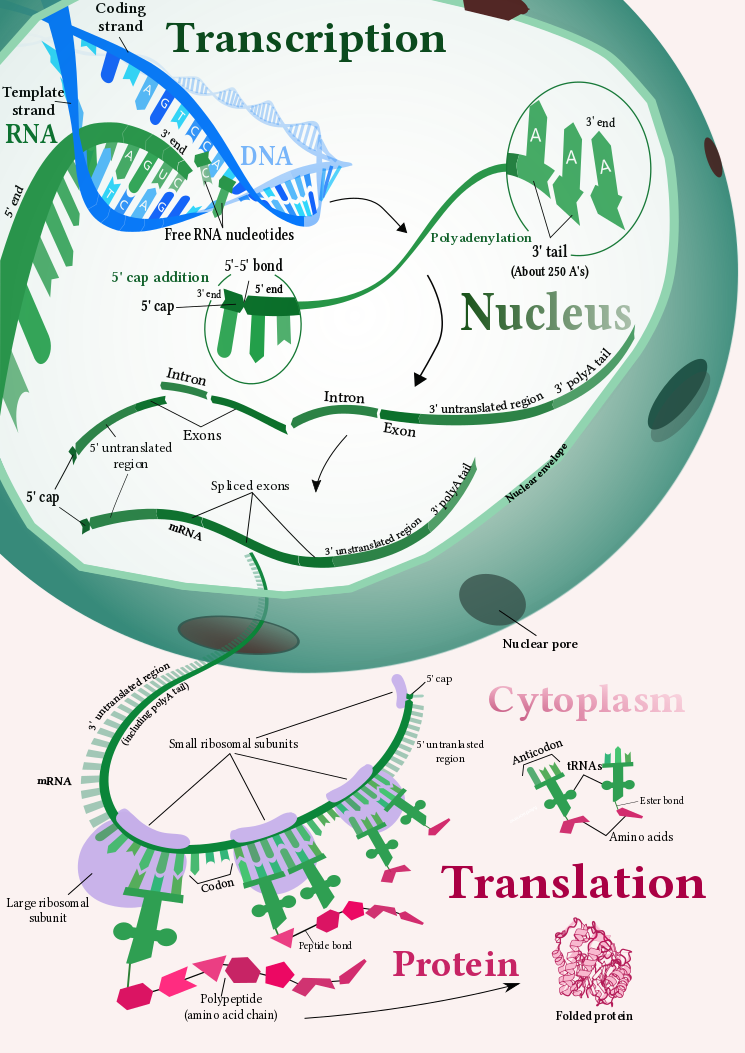
\includegraphics[scale=0.60]{background/transcriptionTranslation.png}\centering
    \vspace{-2.3mm}
    \caption[Transcription and Translation: an overview]%
    {\label{fig:transcriptionTranslation}\textbf{Transcription and Translation: an overview.}
    {\small This work, \enquote{Transcription and Translation: an overview},
    is a derivative work of
    \href{https://commons.wikimedia.org/wiki/File:MRNA.svg}{\enquote{Simplified diagram of mRNA synthesis and processing. Enzymes not shown.}}
    and
    \href{https://commons.wikimedia.org/wiki/File:Protein\_synthesis.svg}{\enquote{Protein synthesis}}
    both by \href{https://commons.wikimedia.org/wiki/User:Kelvinsong}{Kelvinsong},
    used under \href{https://creativecommons.org/licenses/by/3.0/}{[CC BY]}
    (see \Cref{sec:kelvinsong}).
    \enquote{Transcription and Translation: an overview} is licensed under
    \href{https://creativecommons.org/licenses/by/4.0/}{[CC BY]} by Mitra P. Barzine.
    }}
\end{figure}

The transcription initiation happens when
an \gls{RNA} polymerase attaches to the start of the gene
and uses the \gls{DNA} strand as a template
to create a corresponding \gls{RNA}
from free \gls{RNA} nucleotides~\mycite{molBiolCell}.
The transcription is a directional process and
always happens from the gene 5' end towards its 3' end~\mycite{Callen2005-ik}.
(For 5' and 3', see \Cref{fig:DNARNAstruct} and related section.)
Messenger \glspl{RNA} (\glspl{mRNA}) are \glspl{RNA} that are produced from a gene
and used as a template for translation to synthesise proteins.
There are other kinds of \glspl{RNA},
\eg\ \glspl{rRNA} (which are the most numerous \glspl{RNA} in the cell),
\glspl{tRNA} and many others~\mycite{Callen2005-ik}.
The entire repertoire of transcripts (\ie\ \gls{RNA} molecules) expressed
in a cell or group of cells (such as in a tissue)
is called transcriptome~\mycite{Velculescu1997-rs,Pietu1999-uf,rnaseq-2009}.
Unlike the genome which is roughly identical
regardless which cell of a particular individual is considered,
the transcriptome may vary, sometimes dramatically,
according to the biological context (different organs or tissues,
or different conditions, \eg\ healthy or in a reaction to a disease)
and through time and life stages.~\mycite{molBiolCell}\mybr\

Before the \mRNA\ is in turn used as a template to make the protein,
a few modifications may occur.
Among the typical post-transcriptional regulations,
there are
the capping and the addition of a polyadenylated (polyA) tail
(both increasing the half-life of the \mRNA),
splicing
(where internal parts of the \mRNA\ ---
either non coding (\ie\ \emph{introns}) or coding (\ie\ \emph{exons}) --- are removed),
or \gls{RNA} editing~\mycite{Darnell2013-xf}.
For eukaryotic species (\eg\ \species{Human}),
the \mRNAs\ have to be exported
from the nucleus to the cytoplasm for the next step to happen~\mycite{Callen2005-ik}.\mybr\

The \glspl{mRNA} initiate the translation,
\ie\ creation of new proteins,
by binding to protein factories called ribosomes
(complexes formed from \glspl{rRNA} and ribosomal proteins).
The ribosomes read the \mRNA\ codons (\ie\ groups of three consecutive bases)
and produce the corresponding protein by synthesising a polypeptide chain
from the free amino acids (\glspl{aa}) carried by \glspl{tRNA}
with the corresponding anticodons (\ie\ complementary sequence to the \mRNA\ codons).
The \glspl{aa} are linked by peptide bonds formed
through the reaction of functional groups on their primary chain:
the carboxyl group (--\chemForm{COOH}) of the first amino acid \gls{aa}
with the amine group (\chemForm{NH_2}--) of the next one.
This succession of primary chains and peptide bonds constitutes
the protein backbone.
This sequence is by convention described
from the free amino group of the first \gls{aa} (\ie\ N-terminal)
to the free carboxyl group of the last \gls{aa} (\ie\ C-terminal).\mybr\

Once the polypeptide chain is completed,
it folds into a three-dimensional structure,
which is essential for fulfilling its role~\mycite{Morris2016-qv}.
Many proteins need to undergo post-translational modifications (\glspl{PTM})
before being functional.
\glspl{PTM} allow the regulation of the proteins' activity
(activation and deactivation).
They can involve the creation of new covalent bonds,
as many proteins comprise more than one polypeptide chain to be functional.
Other frequent \glspl{PTM} include the phosphorylation, acetylation,
or glycosylation of the \glspl{aa} (also called residues)~\mycite{molBiolCell,Morris2016-qv}.
Besides the variety of possible \glspl{PTM} and their combination,
proteins can comprise twenty different \glspl{aa} (\Cref{sec:aa}),
which have a vast range of physicochemical properties.
Hence, in turn, the proteins have a wide physicochemical range too.
\mycite{Morris2016-qv,Callen2005-ik}.\mybr\

Although the diversity of the proteome
(\ie\ entire repertoire of expressed proteins)
is the primary contributor to
the ending \gls{phenotype}\footnote{Phenotype: \glsentrydesc{phenotype}}
and functions of cells and tissues,
its exhaustive study remains particularly challenging.
Most proteins are quite stable,
but their physicochemical diversity prevents
the use of uniformed and straightforward protocols
that would encompass all the proteins
in a given cell or tissue type.~\mycite{Bruce2013}\mybr\

\begin{figure}[!htbp]
    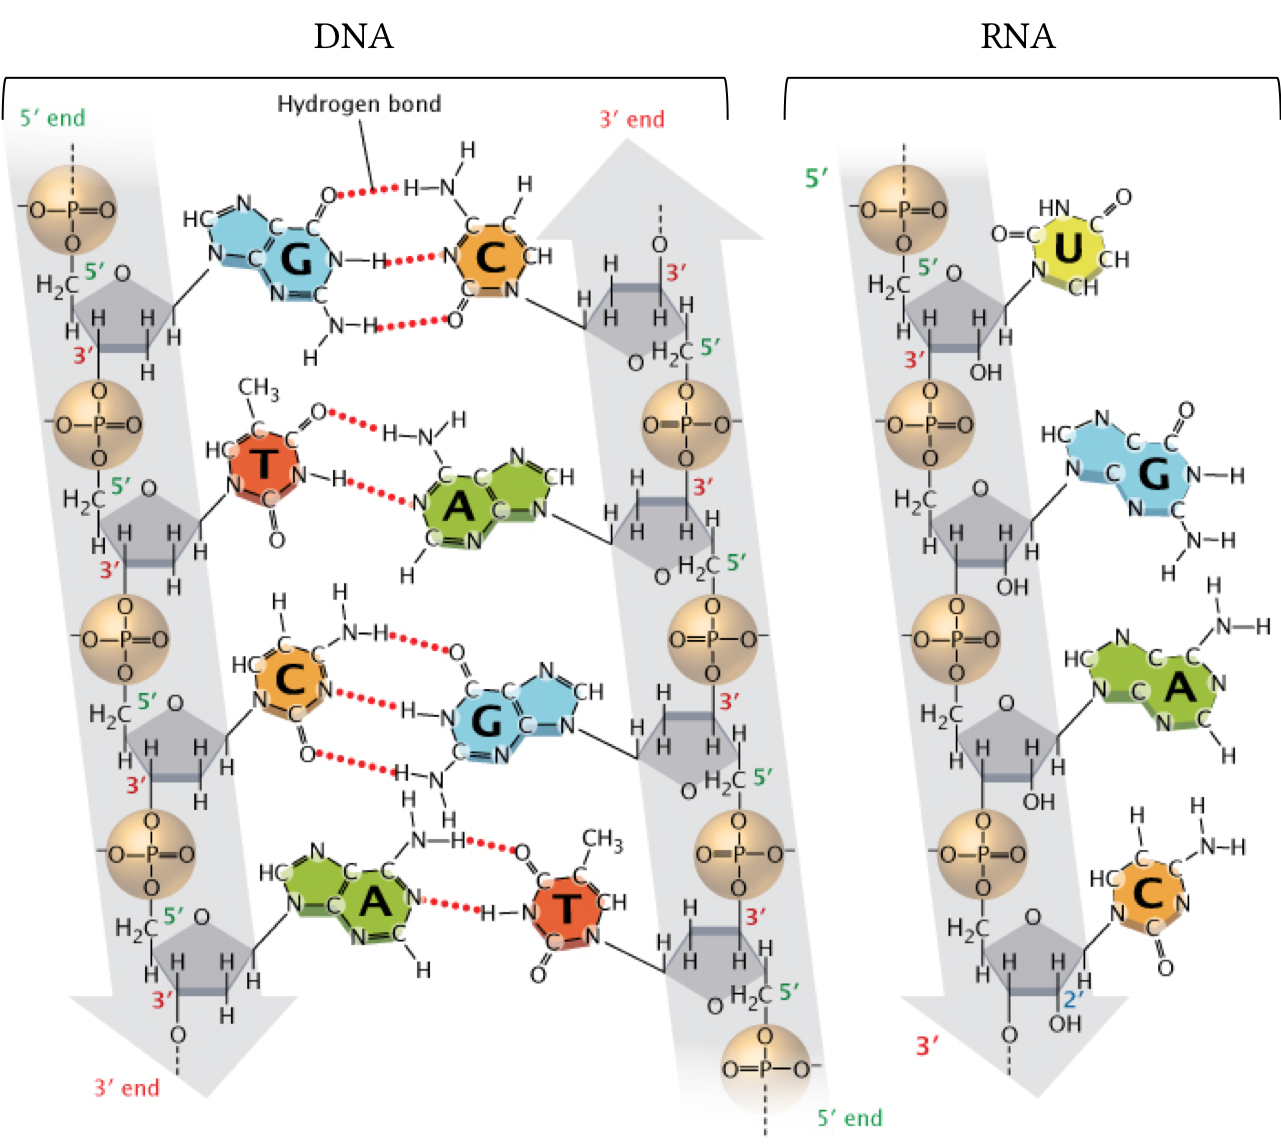
\includegraphics[scale=0.49]{background/DNA-RNAstruct1.png}\centering
    \vspace{-2mm}
    \caption[DNA and RNA structures]{\label{fig:DNARNAstruct}%
    \textbf{DNA and RNA structures} © 2014 Nature Education ---
    Adapted from \citet{Pierce2005-ib}.}
\end{figure}

On the other hand,
all \gls{DNA} and \glspl{RNA} have very similar chemical properties,
as their structures are very close as shown in \Cref{fig:DNARNAstruct}.
They are polymeric molecules that are made by a chain of nucleotides.
Nucleotides have three distinct chemical subunits: a phosphate group,
a pentose (either ribose for \gls{RNA} or deoxyribose for \gls{DNA})
and a nitrogenous base, which can be a purine (adenine (A) or guanine (G))
or a pyrimidine (cytosine (C) and
either thymine (T) for \gls{DNA} or uracil (U) for \gls{RNA}).
The alternation of phosphate groups and the pentoses create the biomolecules backbone,
while the information is encoded into the nitrogenous bases sequence.
\gls{DNA} and \glspl{RNA} all share the same directional reading frame,
\ie\ 5' end to 3' end, or in other words,
from the phosphate group that is linked to the pentose carbon annotated 5'
to the phosphate group
that is linked to the pentose carbon annotated 3'\footnote{%
Pentoses are monosaccharides containing a chain of five carbons.
When the pentose is part of a nucleotide,
these carbons are annotated from 1' to 5' to avoid confusion
with the carbons of nitrogenous cycles.}.~\mycite{Morris2016-qv,molBiolCell,Callen2005-ik}\mybr\

The difference in physical properties between \gls{DNA} and
\gls{RNA} molecules is primarily due to
the predominantly particular arrangement of \gls{DNA} (double-stranded) and
\gls{RNA} (single-stranded).
The double-stranded configuration of the \gls{DNA} dramatically improves
the stability of the \gls{DNA} by involving many mechanisms,
which includes many hydrogen bonds
(three for each couple of G/C and two for each A/T).
Besides,
in eukaryotic cells,
while the genome (\gls{DNA}) is protected in organelles such as the nucleus,
most of the \mRNAs\ life is spent in the cytoplasm,
which contains many enzymes (\eg\ endonucleases and exonucleases)
that cleave the nucleotide sequences and can ultimately degrade the \mRNAs.
Thus, even though \mRNAs\ half-lives are quite variable,
the \mRNAs\ have generally the lowest stability
when compared to the \glspl{DNA} and proteins.~\mycite{molBiolCell,Pierce2005-ib}\mybr\

\begin{figure}[!htbp]
    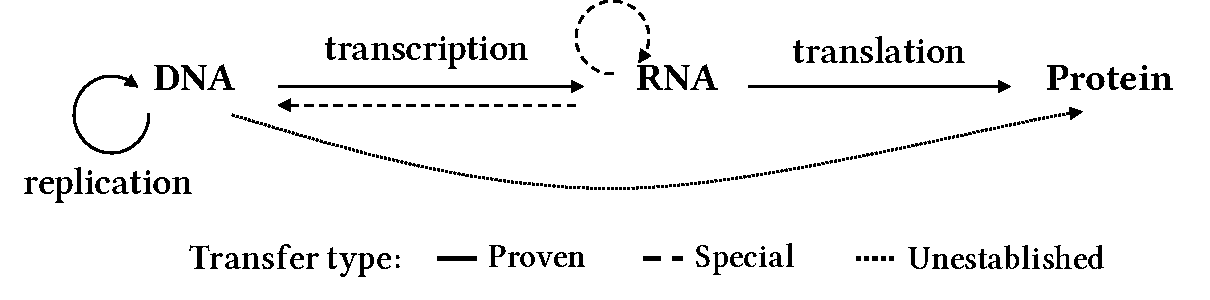
\includegraphics[scale=0.60]{background/dogma.pdf}\centering
    \vspace{-4mm}
    \caption[Central dogma of molecular biology proposed by F. Crick]%
    {\label{fig:dogma}\textbf{The central dogma of molecular biology proposed by
    F. Crick}. The proven modes of information transfers are for the general ones
    in solid lines and in dashed lines for the special transfers
    (\gls{RNA} to \gls{RNA} or \gls{DNA}) and the transfers that have yet to
    be established (\gls{DNA} to protein).
    }
\end{figure}

This overall process, which allows the creation of the proteins and
based on a flow of information initiated from the \gls{DNA},
had been foreseen by Francis Crick~\mycite{Crick:1958,Crick:1970}.
He stated what is now known as the core of the central dogma of molecular biology
(shown in \Cref{fig:dogma}):
\textquote{Once information has got into a protein it can’t get out again}.
In other words, the genome contains all the information needed to produce
functional proteins,
and in theory, if we reach a total understanding of the information encoded
into the \gls{DNA},
we will be able to predict the \gls{phenotype} due to the proteome.
As \gls{DNA} is static
while the coding portion (about 2\%) of the human genome~\mycite{Venter2001-sn}
varies in expression (both in concentration and composition)
depending on the tissue or cell type,
genome studies are easier than transcriptomic or proteomic ones,
but the latter ones are more biologically insightful.\mybr\
\begin{comment}
There are different types of proteins: ubiquitous ones
(generally qualified as \emph{housekeeping}),
cell/tissue/condition specific ones and
everything in-between.
\end{comment}

\section[Transcriptome exploration with RNA sequencing]%
{Transcriptome~exploration~with~RNA~sequencing}\label{sec:transExplo}

With the recent era of short-sequencing technology and the completion of the
Human genome~\mycite{Venter2001-sn,Lander2001-wj,%
International_Human_Genome_Sequencing_Consortium2004-hr},
understanding the genome expression is increasingly a more
reachable aim.
From the early 1980s,
technologies involved in transcriptome studies
have substantially improved through many successive innovations~\mycite{Lowe2017-kj,Parkinson2009-pj}
that include Sanger sequencing~\mycite{Sanger1975-io} or
\gls{PCR} (reviewed by \citet{VanGuilder2008-xs}).
Among the various transcriptomic study approaches,
there are three key methods~\mycite{Lowe2017-kj}:
\gls{EST} sequencing (for gene discovery --- see \Cref{sec:EST}),
microarrays (for gene quantification --- see \Cref{sec:microarray})
and, the one with which all the transcriptomic data used in this thesis have
been generated:
\Rnaseq\ (which is both used for gene discovery and gene quantification).\mybr\

In the following section,
I introduce the typical steps of the required workflow
to study the transcriptome through sequencing on an Illumina platform.
While not by conscious design, all the transcriptomes analysed in this thesis are
the product of Illumina sequencing (see
\Crefrange{subsec:castlepresentation}{subsec:gtexPresentation}).
It is unsurprising as Illumina is by far
the most popular platform for the last decade \mycite{popularIllumina} and
have been used to generate most of the data in \gls{ENA} and \gls{ArrayExpress}.
Indeed, Illumina sequencing offers a very
good balance between accuracy and achieving the highest
throughput for the lowest per-base cost \mycite{IlluminaCheap}.
I will emphasise the approaches and
the tools I used to estimate the gene expression levels from raw nucleotide
sequences.
\Cref{fig:OverviewRnaseqPrepSeq} presents an overview of the typical steps of an
\Rnaseq\ workflow from the libraries preparation to the sequencing.\mybr\

\begin{figure}
    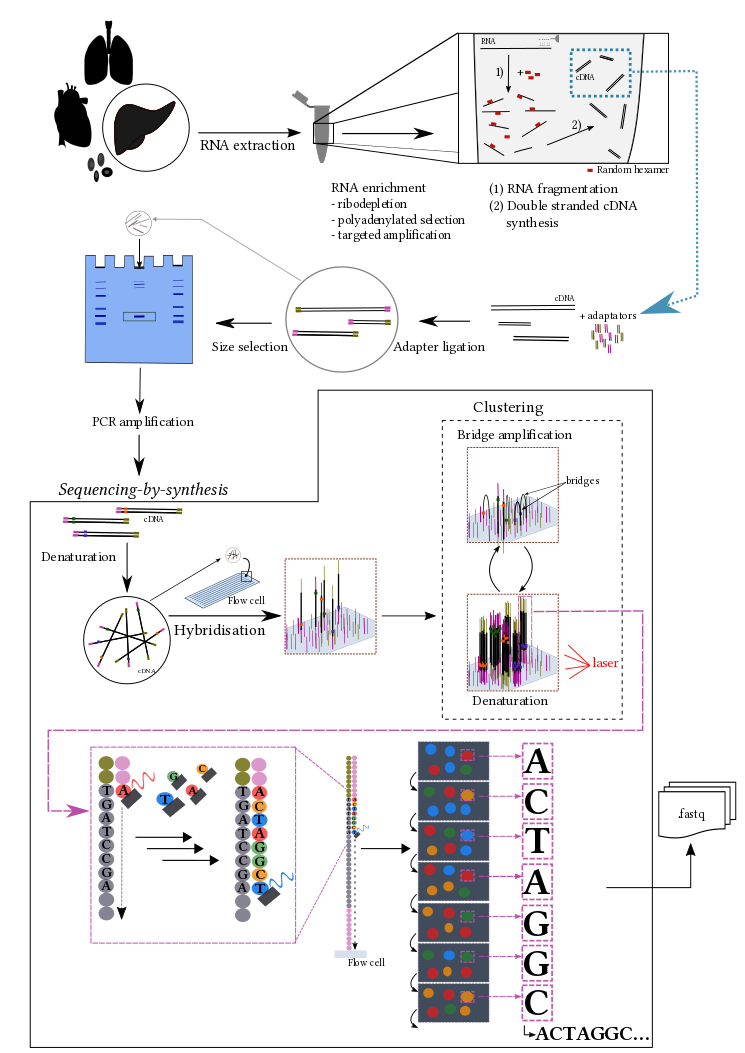
\includegraphics[scale=0.60]{background/IntroWorkflow.png}\centering
    \caption[Overview of a \Rnaseq\ workflow: library preparation
    and sequencing]{\label{fig:OverviewRnaseqPrepSeq}\textbf{Overview of
    a typical \Rnaseq\ workflow:
    library preparation and sequencing}}
\end{figure}

Experimental protocols for other platforms may need various and specific
modifications that are outside of the realm of this thesis and thus will not be
covered here\footnote{More details on the other main sequencing platforms and their
relevant protocols may be found in~\citet{rnaseqProtocols} review paper or at the
online resource \enquote{\href{http://rnaseq.uoregon.edu/}{RNA-seqlopedia}}
(\href{http://rnaseq.uoregon.edu/}{http://rnaseq.uoregon.edu/})
\mycite{rnaseqlopedia}.}.\mybr\

Although the collection and the conservation\footnote{E.g.\ between fresh-frozen
samples and \gls{FFPE} samples see~\citet{sampleConservationMatters}.}
of the samples before the
\gls{RNA} extraction most definitely affects the final estimations,
I will set aside these steps from my review.\mybr\

\subsection{Library preparation}\label{subsec:libPrep}

While there are sequencing technologies that can directly sequence \glspl{RNA}
(see~\cite{rnaDirectSeq}), most of the technologies handle only \gls{DNA}.
Hence, the first step of a typical \Rnaseq\ workflow is the preparation of
\gls{cDNA} libraries from the starting material. This step and the sequencing
itself are the most platform dependent parts of the overall protocol.
Indeed, contingently upon which sequencing principle they rely,
the sequencers need the libraries to be fixed and loaded differently.\mybr\

\subsubsection{\gls{RNA} extraction}

There are many methods to extract \glspl{RNA} from the primary samples, and they
are commonly standardised. Indeed, regarding the type of biological samples,
the \glspl{RNA} of interest, the aim of the  study and the sequencing platform
used, there is one (or more) available commercial kit. These are designed in
a way to not interfere
with any of the later steps of the library preparation or with the sequencing
itself.\mybr\

Without surprise, the choice of one kit (and hence its method of extraction)
over another can impact the final \Rnaseq\ data. The main difference between
the most widespread methods being the quantity of non-mature \glspl{RNA}
(\ie\ with longer intronic regions) detected whereby kit has been used.
However, the relative gene expression levels are similar from one extraction
protocol to the other. \mycite{RNAextraction}\mybr\


\subsubsection{\gls{RNA} enrichment}

After extracting the \gls{RNA} from the cells or tissues,
the next step is to enrich the content of the samples with the \glspl{RNA}
of interest (\ie\ the concentration of the \glspl{RNA} of interest is increased
either by specifically selecting it or by removing other \glspl{RNA}). Indeed,
the \glspl{rRNA} are the most abundant type of \gls{RNA} in any cell. Even
though they account for a very small part of the genome\footnote{For example,
\species{Homo sapiens}, there are 568 genes (<1\%) that are described as
\gls{rRNA} out of the 63,898 annotated genes of the \gls{Ensembl} database
(\hg{38.p10}, \ens{89}).}, they represent by their number 70\% or more of
the total population of \gls{RNA} \mycite{biochbook}.
Although there are interests to study \glspl{rRNA} (\eg{}~\cite{rrnaStudy}),
\mRNAs\ studies are more popular,
and they only constitute about 3 to 5\% of the whole \gls{RNA} population
\mycite{molBiolCell}. Other studies research even scarcer kinds of
\gls{RNA}.\footnote{Out of the 10,081 experiments tagged as \comp{\enquote{rna
assay}} and \comp{\enquote{sequencing assay}} within \gls{ArrayExpress},
7,981 were also tagged as \comp{\enquote{RNA-seq of coding RNA}},
1,829 as \comp{\enquote{RNA-seq of non coding RNA}} and 366 have both tags.
4 of them are only described as \comp{\enquote{microRNA profiling by
high-throughput sequencing}} --- Query date: 22 June 2017.}\mybr\

There are typically three strategies to achieve \gls{RNA} enrichment:
either by polyA-selection, by ribodepletion or (more complex)
by targeted amplification. While these
approaches are insufficiently specific to select one particular kind of \gls{RNA}
or remove all \glspl{rRNA}, it eases and improves the downstream analyses.\mybr\

\minisec{PolyA-selection}\label{msec:polyA}
This strategy essentially targets the \mRNAs. It exploits the polyadenylated
tail at the 3' end of the \mRNAs\footnote{And a few other kinds of \gls{RNA},
\eg\ \glspl{lncRNA} \mycite{polyAlncRNA}} that is added
post-transcriptionally.
Magnetic beads, supporting short strings of thymine (oligo-dT),
capture these \mRNAs\ efficiently while the others
are washed away \mycite{Mortazavi2008}.\mybr\

This protocol is probably the most widespread one as it is the easiest and
cheapest to set up. A dataset produced following this protocol is known as
a \emph{polyA-selected} dataset.\mybr\

\minisec{Ribodepletion}
This strategy is preferred for the study of any \gls{ncRNA} or when researching
the interaction of \mRNAs\ with other \glspl{RNA} \mycite{ribodepletion}. This
strategy is in a way the reverse of the previous one as its also
uses magnetic beads, but this time to efficiently\footnote{ThermoFisher claims
that its RiboMinus protocol can remove till 99.99\% of the \glspl{rRNA}.}
target the unwanted \glspl{rRNA} as to remove from the sample.\mybr\

The ribodepletion can also be achieved through ribonucleases. These enzymes
specifically digest \glspl{rRNA}, and then \glspl{RNA} of interest can be retrieved
through size selection.\mybr\

Datasets produced following a ribodepletion protocol are usually called
\emph{whole \gls{RNA}} or \emph{total \gls{RNA}} as a contrast to the
\emph{polyA-selected} ones.\mybr\

\citet{castleData} created a total \gls{RNA} dataset, but they use another
approach where they amplify \emph{every} other \gls{RNA} with the help of
specially designed probes (see \Cref{subsec:castlepresentation}). Hence,
the protocol they have used is closer to the following one.\mybr\

\minisec{Targeted amplification}
Targeted amplifications rely on primers that would be designed to target (or
avoid as for~\citet{castleData}) specific sequence motifs of the genome.
Most studies based on this kind of approach are referred with
a name based on the studied \gls{RNA} type (\eg\ \gls{miRNA-Seq}) or
emphasising the variation of the method (\eg\ Capture-Seq
\mycite{captureSeq}).
Often,  additional steps are required to prepare the libraries
in comparison with a polyA-selected or ribodepleted dataset.\mybr\

\subsubsection{RNA fragmentation}

Most of the sequencing platforms\footnote{As for the Illumina platforms that have
produced the transcriptomic datasets studied in this thesis.} require relatively
short (\ie\ 200 to 500\ nt) length to sequence. Concomitantly, it also ensures
a more uniform sampling along the \gls{RNA}.
This fragmentation can be carried out via divalent cations hydrolysis or
nebulisation.\mybr\

This step is performed on occasions after the \gls{cDNA} synthesis
(see next section). In those case, the \glspl{cDNA} are fragmented mostly
by digestion with DNase I or by sonication.\mybr\

\subsubsection{Double-stranded cDNA synthesis}
The \gls{RNA} molecules are used as a template for a retro-transcription
involving oligo-dTs or \emph{random} hexamer primers, respectively only
for polyA-selected datasets or any dataset (polyA-selected included).
The set of \emph{random} hexamer has been designed to cover the whole
transcriptome. Unfortunately, these \emph{random} hexamer primers have been
proven to lack full randomness \mycite{notSoRandom}.\mybr\

At the end of the most common protocol, the order of synthesis of each \gls{cDNA}
strands is lost, \ie\ it is impossible to distinguish which of the \gls{cDNA}
strands has the same sequence than the original \gls{RNA}. Several techniques,
called \emph{strand-specific}, have been developed to compensate for this
\mycite{strandSpecific,strandSpe}.\label{strand-specific}\mybr\

\subsubsection{Adapter~ligation,~PCR~amplification~and~size~selection}

After generating blunt edges by restriction digest of the \glspl{cDNA}, adapters
(small known sequences of oligonucleotides) are ligated to their both ends.
These adapters are constituted from several parts. A subset of them are ensuring
later the hybridisation of the \glspl{cDNA} with the flow
cells\footnote{\Gls{flow}: see \Cref{sub:HybridClustAmp}.} (based on sequence
complementary), and another set of them
are sequence binding sites that are used as primers for the following cluster
amplification step occurring \latin{in situ}. These adapters are also used to
introduce additional motifs such as indexes.\mybr\

The next two steps can be interchanged regarding the amount of starting material
at disposition. \gls{PCR} amplifies all the molecules before (or after)
a size-selection is performed (per gel electrophoresis) to extract
length-complying fragments (about 200 to 500\ bp) to the sequencer machine
requirements\footnote{Indeed, the previous fragmentation step creates a great
length range of fragments.}.\mybr\

Unfortunately, the size-selection means that any
transcript with an original length below the threshold used for the
selection will be missed\footnote{There is no problem for the greater length
as they will statistically present fragments that will be in the correct range.}.
For example, \glspl{miRNA} are shorter than the general requirement of Illumina
sequencers. Alternative protocols are addressing this issue
\mycite{smallRNAprotocol}.\mybr\

\subsubsection{An example of alternative preparation strategy}
Along with the targeted, the strand-specific and small \glspl{RNA} protocols,
there are a few other variations to this typical protocol to handle other concerns.
For example, it is occasionally necessary to sequence simultaneously (in a single
run) multiple samples. This can either be motivated by practical reasons
(to lower the experimental costs or hasten the overall processing time)
\mycite{multiplexCheaper} or be critical to the experimental design as a way to
experimentally handle the \emph{batch effects}\footnote{Batch effect: see
\Cref{sub:BatchEffect}} \mycite{multiplexBatchEffect}. However, it is
crucial to later extricate the several pooled samples from each other as a
requirement to many downstream analyses.\mybr\

\emph{Multiplexed} protocols easily achieve
the distinction between the multiple samples as they incorporate \emph{barcodes}
before ligating the adapters. These barcodes are also small sequences of
nucleotides, and each sample has its unique associated
barcode. In practice, each sample is prepared separately with the added extra
step (before the adapters ligation) where the barcode is incorporated; then all
the samples are pooled together before the next step, which consists of hybridising
the \glspl{cDNA} to the flow cell.\mybr\

Other extra steps occur just after the sequencing and before any other data
analysis: all the reads\footnote{Reads: see \Cref{subsub:sequencing}} are
separated in files based on their barcodes and the barcode, along with the
adapters, is trimmed from all the reads.\mybr\

The main inconvenient of the multiplexing protocol is that the original sequenced
length of the \glspl{cDNA} are then shorter as the barcodes are also (and have
to) be sequenced as well.\mybr\

\subsection[Clustering: Hybridisation and Bridge amplification]{Clustering:
Hybridisation and Bridge amplification~\small{\mycite{IlluminaYoutube}}\quad}%
\label{sub:HybridClustAmp}

\vspace{-4mm}
Once the libraries are ready, they are loaded onto a \emph{flow cell}\footnote{%
\emph{Flow cells} are the support of Illumina sequencing. They enable the
parallelisation of the sequencing of millions of \gls{DNA} fragments together
which are kept spatially separated in clusters. This was allowed with the advent
and optimisation of supported Chemistry. Each flow cell is a glass slide with
lanes. Each lane is coated with two short nucleotide sequences. One of these
oligonucleotides is complementary to a region contained in the ligated adapters.}.\mybr\

The clustering step comprises two phases: hybridisation and bridge amplification
of the \gls{cDNA} fragments.\mybr\

\subsubsection{Hybridisation}

The double-strand \glspl{cDNA} are denatured, and then each fragment randomly
hybridises across the flow cell surface with one of its small oligonucleotides.
These are used as primers for polymerases which create a first complementary
strand to the hybridised \gls{DNA} fragments. The new double-strand molecule is
denatured, and the original first template is washed away.\mybr\

\subsubsection{Bridge amplification}
The strands then fold over and their (second) adapter hybridises with a
complementary oligonucleotide sequence of the flow cell and thus creating a
bridge. The flow cell complementary fragment is then used as the primer for a new
strand. The new double-stranded \gls{DNA} is then denatured (which
dismantles the bridge). Each of the two tethered molecules creates a new
bridge by hybridisation which are the templates for a new strand each.
This process happens many times and simultaneously for millions of fragments.
It creates clusters of clonal amplification of the original fragments of
the library. After the bridge amplification, the reverse strands are cleaved
and washed away. The 3' end primers are also blocked to avoid any unwanted
priming.\mybr\

\subsection{Sequencing-by-synthesis}%
\label{subsub:sequencing}

Illumina sequencers propose two sequencing approaches: single-end and paired-end.
The difference is that in \emph{single-end sequencing}\footnote{Chronologically
the oldest method}, the sequencing begins at one (and only one) of the fragment
ends and progresses towards the second. Whereas in \emph{paired-end sequencing},
once the first end has been sequenced (as in the single-end approach), after a
single new bridge replication, the other end of the original fragment is
sequenced as well.
Hence, with a small change in the original single-end adapters~\mycite{pairedEndAdapters},
in paired-end protocols, the sequencing occurs at \emph{both}
ends of each original fragment.\mybr\

Though more expensive and more challenging to programmatically handle,
the paired-end approach produces more information and hence facilitates
the detection of genomic rearrangements (as indels or inversions) and
repetitive sequence elements.
It also allows an easier distinction between isoforms of the same gene and provides
greater support to detect the novel transcripts (new isoform or new gene) and fusion
genes\footnote{A \gls{fusionG} is a gene that is the product of the fusion of
parts of two (or more) different genes.}.\mybr\

In both cases, the sequencing process is the same. It is an Illumina proprietary
process, and it is called \emph{Sequencing-by-Synthesis}~\mycite{seqBySynth}.
It uses the \gls{DNA} replication mechanism with modified \dNTPs.
It relies on the step-by-step incorporation of
reversible fluorescent tagged \dNTPs\ who are protected at
their 3'end to block any further elongation.
The product of this synthesis is called a \emph{read}, and
it supports the \emph{base calling}\footnote{Base calling:
identification of the nucleosides in a sequence
by assigning chromatogram peaks
or another kind of signal variations
to (nucleo){}bases.}.\mybr\


The sequencing co-occurs on every identical fragment
of every cluster of the flow cell.
It begins with the hybridisation of a complementary 5' primer onto the 3' binding
site of the tethered \gls{DNA} template. This primer is then extended by
replication to create a new read. Next, the sequencing cycle (described below)
repeats itself several times.\mybr\

The \emph{sequencing cycle} starts with the addition of one complementary
fluorescent \dNTP\ to the new growing read, and
the replication process stops since the \dNTPs\ are blocked at their 3' end.
Afterwards, all the unlinked
\dNTPs\ are washed away. Then, the clusters are excited by a light source,
and as each
\dNTPs\ has a fluorescent tag with its own characteristic wavelength, the
signal that they emit back will allow \emph{calling} (\ie\ identifying) what is the
new nucleotide that each cluster has incorporated. The signal intensity and
its wavelength are recorded (both of them are needed for the base calling
process for the base call itself and its associated accuracy). Finally,
the fluorescent tags and the 3' caps are cleaved
and washed away so a new cycle can happen.
The number of cycles determines the final length of the reads.\mybr\

Unfortunately, as the sequencing proceeds, the error rate of the sequencers
increases. This is due to the incomplete removal of the fluorescent signal which
increases the background noise and thus reduces the signal-to-noise ratio.\mybr\

Once the programmed read length is achieved (typically between 25 to 200 \gls{nt}),
the reads are washed away (after denaturation).\mybr\

\subsubsection{Sequencing specificities for the \emph{paired-end} protocol}

Then, after the introduction of a new primer, the first index is sequenced
following the same sequencing cycle.
Once completed, the index read is washed off, and the 3' end primer is deprotected.
Then, the \gls{DNA} fragment bends over and hybridises to a complementary
oligonucleotide at the surface of the flow cell.
Next, the second index is sequenced, and its product read washed away,
a single new bridge replication follows.
The new double-stranded \gls{DNA} fragment is denatured, and the 3' primers are
protected before the forward strand is cleaved and washed away.
Finally, the reverse strand is sequenced following the previously described
sequencing cycle. Once the same number of sequencing cycles than the forward
strand is reached, the read product of the reverse strand is washed away.\mybr\

\subsection{From analogous input to digital output}

At the end of the sequencing process, the set of images (one per sequencing cycle)
is produced. While it is possible to work with the images themselves, in most
cases, the sequencing facilities will perform the base calling and provide the
end-user with text files. In single-end sequencing, there is one file per sample.
In paired-end sequencing, the reads are usually separated based on their associated
indexes into two ordered files: all the reads from the forward strands (one end)
are grouped in one file, and the ones from the reverse strands (other end)
in a second one.\mybr\

These files are usually distributed in the \fastq\ format~\mycite{fastqFormat}
which record for each cluster (read) a unique identifier,
a nucleotide sequence and a \gls{Phred} quality score for each base of the
sequence. A few optional information can also be provided, \eg\
the position of the read on the \gls{flow} (See \Cref{sec:fastq-format} for
a random read example).
The \gls{Phred} quality score ($Q$) measures the accuracy of the identification
of the nucleobase to which it refers. These scores are set by the base calling
program and are defined as $Q = -10\log_{10}(P)$ with $P$ the probability of
the base being called wrongly. There are several possible encoding formats
(see \Cref{sec:PhredScore}).\mybr\

\subsection{A typical bioinformatic workflow for \Rnaseq\ study\quad}\label{sub:RNAseqworflow}

From the reconstruction of the
transcriptome to the normalisation of expression in each sample, the various
steps may be addressed through many different algorithmic approaches.
Often, the choice of a method at one stage implies a more limited number of
alternatives from which to pick at later points in the pipeline.
The choice is frequently driven by the kind of downstream analyses planned for
the study. More than the practical format of the data for these, it is the
assumptions and the methods used upstream that are critical for a
rigorous investigation and, later, for an accurate interpretation of the results.\mybr\

\Cref{fig:pipelineTrans} presents an example of the overall \latin{in silico}
process of raw \Rnaseq\ data. It summarises the steps and highlights the tools
I used to process the data within this thesis.\mybr\

Before any downstream analysis, for each read, the genomic region (or
\emph{locus}), from which it has been expressed initially, needs to be identified.
Indeed, \Rnaseq\ main objective is to quantify the expression of genomic
\emph{features}\footnote{These genomic features could be genes, isoforms,
exons, novel genes, \dots\
In short, any genomic region with an annotated function.}. In other words,
the transcriptome needs to be reconstructed from the short reads and annotated
(\ie\ identify which features have been expressed in each library).\mybr\

Two different main strategies (see further `Reconstruction strategies' segment)
manage to accomplish this identification step. Independently of the
approach, this step is the most challenging and time-consuming
of the workflow. Tools, which tackle the reconstruction, usually provide
many tunable heuristic parameters (\eg\ maximum number of allowed mismatches
or indels per read before discarding a possible identification\footnote{Indeed,
many reads will have many identifications; these reads are defined as
\emph{ambiguous reads}.})
to speed up the task.
Unfortunately, as on Illumina platforms, the base calling accuracy decreases
along the read length, this may lead to an information loss~\mycite{TrimRNAseq}.
To prevent informative reads to be discarded, it is opportune to perform a quality
check of the raw data before the identification step. Thus, reads with a drop of
accuracy in their 3'end may be shortened (\ie\ trimmed) and rescued for the next
reconstruction step. Similarly, low-quality reads may be discarded hence
lowering the complexity
of the reconstruction task and hasten its accomplishment.\mybr\

\subsubsection{Quality check, trimming and filtering}\label{subsub:trim}

The quality assessment allows removing any read (or part of it) that would
increase the complexity of the reconstruction step or skew the downstream analyses.\mybr\

It is wise to discard uninformative reads, \ie\ reads with a low sequence
complexity (\eg\ poly-T or poly-A tails) or with ambiguous sequences (in other
words with uncalled bases --- reported as \emph{N}).
Indeed, these reads will hamper the processing time as they
usually map to several parts of the genome while also decreasing the accuracy of
the global gene expression estimations.
For similar reasons, it is judicious to remove reads with a low overall quality
score\footnote{It may vary based on the complete set of reads to analyse.}.\mybr\

It is also prudent to check and remove any read that may map to possible
contamination sources\footnote{For example, for eukaryotes, by aligning (see next
segment) every read to the \species{Escherichia coli} genome.}.
Indeed, as these reads are ambiguous, it is safer
to discard them than skew the expression estimations.\mybr\

Finally, as many tools (mappers in particular) only accept reads
with a unique length, the purity-length balance requires optimisation.
Indeed, the trimming has to compromise between
an approach too lenient (where the mappers discard many unfit reads at a later step),
and
a too stringent one (where either the reads are shorter,
which increases the overall complexity and therefore hinder
the mapping both on time and accuracy~\mycite{Trimwisely},
or too few are left for pertinent analyses).\mybr\

Generally, after the sequencer calls the reads, a first trimming removes
all the adaptors and barcodes needed by the sequencing protocols. Thus,
in principle, they are not to be found in the \enquote{raw data}.
However, to avert any latter contingency, a search against
a list of the most common adaptors and an over-representation assessment of small
sequences (\emph{k-mers}\footnote{\emph{k-mer}: In the present context, all
possible subsequences of length
\emph{k} of a \emph{read}.}) at each end of the reads is good practice.\mybr\


\subsubsection{Reconstruction strategies}\label{subsec:reconstruction}

Two main approaches can be used for the very computationally expensive step of
identification. I will present them in decreasing order of complexity:
the \latin{de novo} assembly of the reads and then the reads alignment approach
(to a genome reference or a transcriptome one).\mybr\

Regardless of the approaches, the reconstructed transcriptome is usually reported
as a \emph{\gls{SAM}} file~\mycite{SAMformat} (or one of its derivative formats:
either \emph{\gls{BAM}} or more recently \emph{CRAM}).\mybr\


\minisec{\latin{de novo} Assembly}
This approach is favoured when the reference genome of the species of interest
is unavailable or of poor quality
(\eg\ many non-model organisms) or inadequate (\eg\ cancer samples)
for the samples of interest. However, if a reference already exists this strategy
is avoided to the utmost.\mybr\

It allows the unbiased discovery of novel
exon-exon junctions~\mycite{deBruijn}. As none of the datasets I use in this
thesis has been reconstructed through this approach, I briefly summarise
the main points below as more in-depth reviews cover this strategy
(see~\cite{denovoReview}).\mybr\

In \latin{de novo} assembly, the reconstruction of the transcriptome happens
with the construction of the longest possible \emph{contigs} (\ie\ contiguously
expressed regions) based on sets of overlapping reads (see also
\Cref{fig:denovo}). Shorter reads add
to the overall complexity of this approach. While paired-end reads may help to
solve many genomic regions, lowly expressed or repetitive regions remain
challenging to determine. There are several algorithmic approaches for \latin{de
novo} transcriptome assembly~\mycite{algorithmsDenovo},
though the most prevalent one is the de Bruijn representation~\mycite{deBruijn}.\mybr\

\begin{figure}[!htb]
    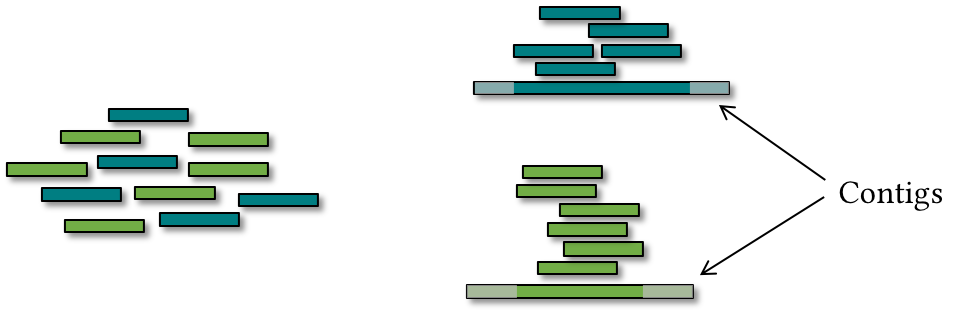
\includegraphics[scale=0.60]{background/denovo.png}\centering
    \caption[\textit{de novo} Assembly]{\label{fig:denovo}\textbf{\latin{de novo}
    Assembly.} From overlapping regions of raw reads, \emph{contigs} are
    created by integrating the reads sequences together.}
\end{figure}

\minisec{Read alignment}
This approach exploits prior knowledge. The reads are aligned to a reference to
hasten the reconstruction process. The reference may be a genome or a
transcriptome (provided that a good annotation is available).\mybr\

\begin{figure}[!htb]
    \centering
    \begin{subfigure}{1.1\textwidth}\label{fig:genoAlignment}
        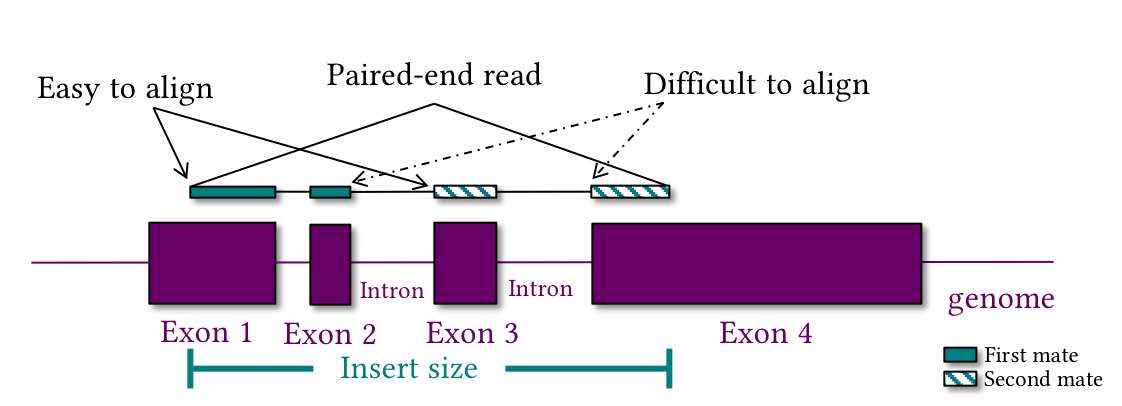
\includegraphics[scale=0.60]{background/genomeAlignment.png}\centering
        \caption{Alignment to the genome}
        %\label{fig:genoAlignment}
    \end{subfigure}

    \begin{subfigure}{1.1\textwidth}\label{fig:transAlignment}
        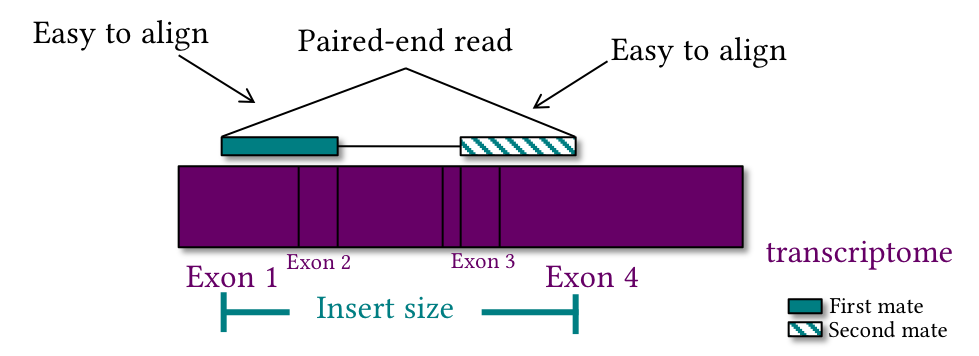
\includegraphics[scale=0.6]{background/transcriptomeAlignment.png}\centering
        \caption{Alignment to the transcriptome}
        %\label{fig:transAlignment}
    \end{subfigure}
    \caption[Overview of main alignment strategies for \Rnaseq\
    transcriptome]{\label{fig:OverviewRnaseqMapping}\textbf{Overview of main
    reconstruction strategies for an \Rnaseq\ transcriptome by alignment to a
    reference}}
\end{figure}

\subminisec{Genome reference}
Aligning to the genome allows discovering new genes or isoforms. However, it
requires splice-aware algorithms, \ie\ they need to align the
reads across the splice-junctions (which is possible but non-trivial).
As illustrated in \Cref{fig:genoAlignment},
the reads might span many discontinued regions of the reference.
While on the one hand, aligning to the genome avoids \emph{multiple mapping
issues}\footnote{Due to sequence similarity, a same read or subpart of a read
may be attributed to many different loci in the genome. As it is
impossible to attribute the read to its original locus of expression directly,
distribution models have to be pondered to avoid unnecessary skewness during
the quantification step.} for the same exon, this also implies that
the genome needs to provide the coordinates for the different isoforms
which will then require further analyses for accurate quantifications at that
isomeric level.
Indeed, irrespectively of the number of isoforms including a specific exon,
the sequence of this exon is transcribed only once in the reference.\mybr\


\subminisec{Transcriptome reference}
Using a transcriptome for reference instead of a genome reduces the complexity
of the aligning step due to the lack of intronic sequences.
However, it also limits the potential downstream analyses,
\eg\ any new (or unannotated) gene or isoform will be missed.
This approach is the easiest, but a pre-existing
accurate and well-annotated gene model is required.
\Cref{fig:transAlignment} shows in fact that this approach is simpler
to the previous one as a direct read alignment is done against the
transcriptome of reference.
This enables the accurate gene isoforms expression quantification,
provided that the gene model is correct and the reads may be
attributed unambiguously to a single isoform for each gene.
However, in practice, this approach produces many multimapped reads,
particularly for shorter reads as
many isoforms are very similar in sequence and vary only in the exons
they retain.
If the difference in the exon compositions is towards the end of the gene,
reads from two isoforms may be indistinguishable.
Paired-end sequencing helps to resolve part of the ambiguity encountered
with single-end protocols.\mybr\

To mitigate between very computational greedy approaches and more constraining
ones, several tools complementary use the previous strategies.\mybr\

\minisec{Hybrid approach between \latin{de novo} and alignment}
There are tools like \toph\footnote{\toph\ ---
\href{https://ccb.jhu.edu/software/tophat/index.shtml}
{https://ccb.jhu.edu/software/tophat/index.shtml}} (2.0.12)~\mycite{tophat2}
(which has been used to reconstruct all the
transcriptomes involved in this thesis --- see \Cref{ch:datasets}),
that uses a hybrid approach between a reference alignment and a \latin{de novo}
assembly. As a first (but optional) step, \toph\ tries to contiguously
align the reads with \soft{Bowtie}\footnote{\soft{Bowtie} ---
\href{http://bowtie-bio.sourceforge.net/index.shtml}%
{http://bowtie-bio.sourceforge.net/index.shtml}}~\mycite{Bowtie}
to the reference transcriptome when this one is provided. Then
(or alternatively as a first step), the unmapped reads are aligned to the
reference genome. The intention in these alignment steps is to identify and
localise the exons, which may eventually span over splicing junctions and be
connected through spliced alignment. Then, \toph\ builds a database of
possible exon-exon splice junctions from the set of mapped reads and then split
the remaining unmapped (or aligned with a low score) reads to smaller segments
in order to find
possible new split events via a seed-and-extend approach. Potential new events
are considered when these smaller segments, first, match exactly the reference
for their good-quality score regions and, secondly, they have overlaps
(for a user-defined length) with a splice junction. These segment sections are
called seeds. Any read with a seed is then checked for a longer or even complete
alignment to the exons on both sides of the junction.\mybr\

In the case of paired-end data, each read of the pair is first processed
separately.
Then, in the final evaluation phase and
with the help of additional information sources,
they are used as a pair to infer among the many possibilities which
are the most credible ones.
Both parts of a paired-end data once aligned to a
concordant region of the genome is then called a \emph{fragment} instead of a
\emph{read}. Today, there is assimilation between the \enquote{\emph{read}}
and the \enquote{\emph{fragment}} terms. Even though the locution \emph{fragment}
is more accurate and may be used in any situation (as it equals to one read for
single-end data and a pair of related reads for paired-end data), it is
frequent to see the denomination \emph{read} instead (even for paired-end data).\mybr\

\toph\ ---
along with \soft{STAR}\footnote{\soft{STAR} ---
\Href{https://github.com/alexdobin/STAR}}~\mycite{STARpaper} ---
is the most popular splice-aware mapper for genomes with a near-complete annotation
(\eg\ for \species{Homo sapiens})~\mycite{tamaraRNA}
although being slower than the latter~\mycite{hisat}.\mybr\



As many concepts or terms in Science, \enquote{\emph{Read mapping}} can
have different (however very closely related) meanings.
Hence, while for many people, \emph{Read mapping} will encompass any
transcriptome reconstruction strategy (including \latin{de novo} assembly) since
the main point is to map the features to functional annotations,
for others the locution will only refer to
`Read alignment' strategies specifically~\mycite{readMappingDef}.
Tools as \soft{TopHat2} contributes to this locution vagueness.\mybr\

\subsubsection{Quantification of \emph{features}}\label{subsubsec:rnaseqQuant}

When working with \Rnaseq\ data, the typical next step after mapping the reads or
fragments to the reference is to quantify the expression of the
feature\footnote{E.g.\ genes, isoforms, exons, splicing events.}
of interest.\footnote{In fact, while genotyping, heredity
studies and other genetically focused studies are possible in principle, the common
main focus is centred on expression estimation. For example, instead of
reporting a specific \gls{SNP}, in an \Rnaseq\ study, the core interest is
currently more about the specific allelic expression. Moreover, most of the \Rnaseq\
studies lack to provide the sequence depth and coverage for other kinds of study.}
In the context of this thesis, I only consider gene expression (either as \gls{RNA}
or as protein). Hence, many subtleties required for isoforms or exons studies are
here irrelevant and are left out of my overall review.\mybr\

Several tools and algorithmic approaches are available.
Indeed, for larger genomes, many regions may present high sequence similarity
which results in many \emph{ambiguous} (and challenging) reads as they mapped to
many potential genomic sites. These reads are also called \emph{multireads}.
One early strategy to solve multireads is to discard them from later analyses;
another one is to attribute them to the most credible locus based on
the overall distribution of the reads for a given sample. \mycite{Mortazavi2008}
Paired-end data help in many cases to discriminate between possible genomic
original sites, thus decreasing the overall number of multimapped fragments.\mybr\

Two popular tools were used in this thesis,
\cuffl\footnote{\cuffl\ ---
\href{http://cole-trapnell-lab.github.io/ufflinks/manual/}%
{http://cole-trapnell-lab.github.io/cufflinks/manual/}} (2.2.1)~\mycite{cufflinks} and
\htseq\footnote{\htseq\ ---
\href{http://www-huber.embl.de/HTSeq/doc/index.html\#}%
{http://www-huber.embl.de/HTSeq/doc/index.html\#}} (0.6.1p1)~\mycite{htseq},
which are both compatible with \toph\ but rely on different concepts.
I briefly present them below in their chronological release.\mybr\

\minisec{Cufflinks}\label{minisec:Cufflinks}
\cuffl\ is part of a collection of tools called
\soft{Tuxedo suite}\footnote{\soft{Tuxedo suite} user group:
\href{https://groups.google.com/forum/\#!forum/tuxedo-tools-users}%
{https://groups.google.com/forum/\#!forum/tuxedo-tools-users}} which also includes
\toph\ and \soft{Bowtie}.
%In fact, the first releases of \soft{TopHat} and
%\soft{Cufflinks} share many common authors, and
\cuffl\ can assemble
\latin{de novo} novel transcripts and isoforms following the same principles
than \toph. Likewise, using good references is faster and more useful.
In both cases, \cuffl\ infers the most parsimonious\footnote{As a requirement to
Occam's razor, which may be a debatable strategy~\mycite{OccamRazorAndBiology}}
and credible set of transcripts (and their isoforms) that can explain the
complete set of observed fragments.\mybr\

This task is challenging as many isoforms are sharing a common set of exons.
While most genes present a dominant isoform for a specific condition,
there are often a few other isoforms expressed along, even though their amount
may be very limited~\mycite{oneDominant}.\mybr\

Furthermore, \cuffl\ tries assigning the multimapped reads to one isoform only.
First, sets of fragments are separated into sets of isoforms
(all fragments that are likely produced from the same set of isoforms
are regrouped together).
Then to estimate the abundance of each isoform of one set,
\cuffl\ integrates many information sources together.
For example, the overall distribution of fragments
(or reads), if these are spanning over known (or novel) splice-junctions.
Particular attention is drawn to the fragments that map unambiguously to one
unique isoform. When available, paired-end fragments are critical:
as they cover longer regions, the probability
that they span multiple adjacent exons is increased which helps to resolve
the possible structure of the original isoforms. \mycite{CufflinksPaper2}\\
The abundance is finally estimated through
an \gls{EM} algorithm~\mycite{EM-what,EM-algo-latest},
with the following main steps (see also \Cref{fig:cuffEstimation}):\mybr\
\begin{enumerate}
    \item \emph{Initialisation}: For each fragment, a rough estimation of the
        probability to be expressed from each isoform is computed based on the
        different piece of information cited previously.
\item \emph{Iteration till convergence with the observed distribution of fragments}:
    \begin{enumerate}
        \item Isoforms abundance are recomputed based on the updated
            fragment-to-isoform assignment
        \item Fragment-to-isoform assignment re-updated based on the isoforms
            abundance.
    \end{enumerate}
\end{enumerate}


\begin{figure}
    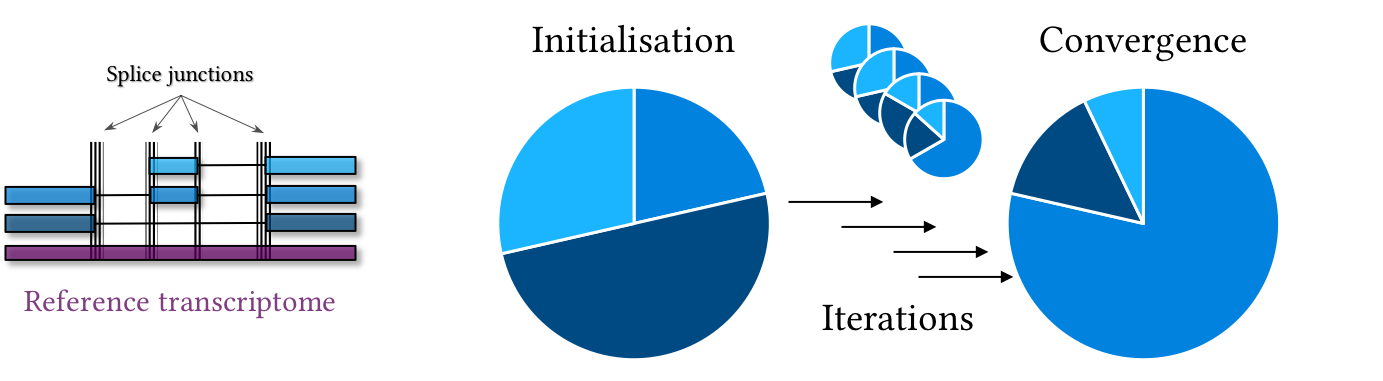
\includegraphics[scale=0.60]{background/CufflEstimation.png}\centering
    \caption[Abundance estimation of isoforms by
    Cufflinks]{\label{fig:cuffEstimation}\textbf{Abundance estimation of isoforms
    by \cuffl} following an \gls{EM} algorithmic approach. [Adapted
    from~\citet{Turner2015}]}
\end{figure}

Finally, to compute the gene expression levels, \cuffl\ aggregates \latin{per}
gene all the isoforms expression abundances together.\mybr\

\cuffl\ provides by default \FPKM\footnote{See \Cref{subsub:norm}.}
\emph{normalised} data.\mybr\

\minisec{HTSeq-count}
The \gls{Python} library \soft{HTSeq} provides a stand-alone script
(\htseq) performing the feature quantification with a more conservative strategy.
It discards all ambiguous reads from a \gls{SAM}/\gls{BAM} file and then
only counts the \emph{un}ambiguous reads that overlap with the features of
interest for a given gene model\footnote{Gene models are distributed as
annotation file (usually either as \gls{GTF} or \gls{GFF} format) and refer
to a specific reference (genome or transcriptome).}.\mybr\

\begin{figure}
    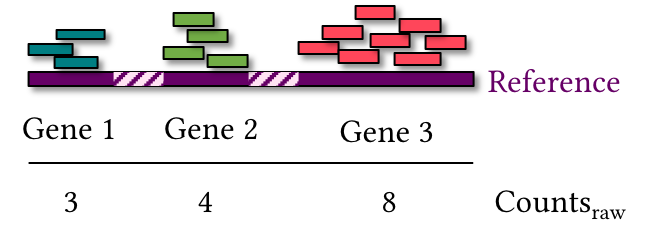
\includegraphics[scale=0.60]{background/htseqQuant.png}\centering
    \caption[Abundance estimation of genes by
    HTSeq-count]{\label{fig:htseqEstimation}\textbf{Abundance estimation of genes
    by \htseq}. The unambiguous reads (or fragments for paired-end data)
    overlapping locus annotated as gene are directly counted. [Adapted
    from~\citet{MarPhD}]}
  \end{figure}

\htseq\ deems as ambiguous any multiread or read that overlaps more than
one annotation for the considered feature.\footnote{In fact, reads might be
discarded for one feature but kept for another one. For example, to quantify the
expression of a given gene, \htseq\ considers every read that unambiguously
overlaps with any of its annotated exons --- indeed, \htseq\ defines a gene
as the union of all its exons. However, while quantifying exon expression, many
of these same reads may be discarded as they overlap several exon annotations
with overlaying definitions.}
\htseq\ provides three modes for fine-tuning the overlap definition.
For this thesis, I used the \enquote{\texttt{intersection non-empty}} mode
(see \Cref{fig:htseqMode}).
This mode avoids discarding too many reads due to a too tolerant annotation
(\ie\ the annotation itself presents many overlapping definitions for a given
pair of feature and chromosome region).\mybr\

Initially, \htseq~\mycite{htseq} was designed for \gls{DGEA}.
This type of analysis compares expression profiles
to highlight the genes (or transcripts)
for which the expression is significantly different
depending on the considered condition.
As multireads are irrelevant for those studies,
including or excluding them from the downstream analysis is insignificant.\mybr\

Interestingly, many papers
(\eg~\citet{Fonseca2014,errorsRNAquant,tophatStarwhatever})
have since shown that
the gene expression estimation by \htseq, while underestimated, is overall
well-correlated with other \gls{RNA} quantification methods
(\eg\ microarrays or \gls{RT-qPCR}).
Moreover, quantifications with \htseq\ are highly correlated with \cuffl\
quantifications for most of the genes after
proper normalisation~\mycite{tophatStarwhatever}
as \htseq\ provides \emph{raw counts} (\ie\ unnormalised counts).\mybr\


\subsubsection{Normalisation}\label{subsub:norm}
Regardless of the quantification method, a normalisation is usually
necessary to avoid a few statistical biases (mainly due to the sampling). The
normalisation method, though, is generally determined based on the quantification
(method or tool\footnote{Many quantification tools (\eg\ \cuffl) perform
the normalisation step automatically as well. They may also (or not) provide
raw counts.}) and they have to be suitable for the planned downstream analyses.
As unfortunately, \Rnaseq\ lacks (still) to assess the real concentration of each
expressed gene (or transcript) in a sample, each normalisation method is based on
a specific set of assumptions that may be incompatible to the ones required by
many investigative approaches.\mybr\

Many papers review or compare normalisation methods (See~\citet{Dillies2013,%
normSigCancerHelp,NormImpact,ruvseqComQN}).\mybr\

\minisec{RPKM and FPKM}
The first evident source of sampling bias is the total number of \emph{mapped}
reads (or fragments) between two \Rnaseq\ libraries (shortened as
\enquote{libraries} from now on). Indeed, there may be considerable discrepancies in
their respective amount of starting material loaded on a
\gls{flow}\footnote{In fact, this would involve the monitoring of many parameters
or assessments of the samples before the library preparation. Moreover, while
it \emph{may} be possible to weight each sample before extracting the \gls{RNA},
the many steps (involving the fragmentation of the \glspl{RNA},
\gls{PCR} syntheses or size-selection) and their associated biases
overburden the tracking of the final amounts used for the sequencing.}
and, more importantly, \emph{the number of mapped reads (or
fragments)} to a reference\footnote{The quantification disregards the
\emph{unmapped} reads (or fragments) and so does the normalisation.}.\mybr\

The second source of bias arises when two genes have their expression level
compared. Indeed, as a longer gene produces more reads (or fragments), it has a
greater statistical chance to be sampled. \Cref{fig:htseqEstimation} illustrates
this sample bias: \frfig{Gene 3} is twice as long as than \frfig{Gene 2}, and their
raw counts also present this scaling factor. However, with proper normalisation,
\frfig{Gene 2} and \frfig{Gene 3} are expressed in equal proportions.\mybr\

To correct for these two biases,~\citet{Mortazavi2008} introduced a new unit
\enquote{RPKM} which they first defined as \emph{Reads} per
Kilobase of \emph{exon model} per Million mapped \emph{reads}.
Since this unit is usually redefined as \emph{Read} per
Kilobase of \emph{transcript} per Million mapped \emph{reads}
and thus, \enquote{FPKM} usually stands for  \emph{Fragments} per
Kilobase of \emph{transcript} per Million mapped \emph{reads}
to also account for paired-end data\footnote{As mentioned before,
despite the inaccuracy, \emph{read} and \emph{fragment} are often used
interchangeably; this is also the case for \emph{\RPKM} and \emph{\FPKM}.}.\mybr\

The canonical formula for \FPKM\ (or \RPKM) is:\mybr\

\begin{equation}
    \tag{Canonical F/RPKM formula}\label{eq:rpkm-fx}
\hat{\mu}_{ij}=\frac{f_i}{F_j\cdot10^{-6} \cdot \ell_i\cdot10^{-3}}
              =\frac{f_i}{F_j\cdot\ell_i}\cdot10^{9} \text{\,}
\end{equation}

where: \\{\small
$\hat{\mu}_{ij}$ is the normalised expression for the \emph{feature} (\eg\ gene or
transcript) $i$ in sample $j$,\\
$f_i$ is the count number of the fragments (or reads) mapped to
\emph{feature} $i$ in sample $j$,\\
$F_j$ is the total count number of all the fragments (or reads) mapped in
sample $j$,\\
$\ell_i$ is the length of \emph{feature} $i$.
}

The scaling factor was introduced such as in most cases $1$\ \FPKM\ is
roughly equivalent to $1$\ \gls{RNA} in the cell~\mycite{Mortazavi2008}. This
has been observed in other papers (see for example~\cite{Hebenstreit:2011}) and
also explains why $1$\ \FPKM\ is a commonly used threshold.%eg\citet{Blazie2015-zv}
\mybr\

This normalisation is quite intuitive and still largely used today.
In fact, I use this normalisation through the thesis.
However, it is also unsuitable for
\gls{DEA},
which is a popular type of analysis.
Indeed,
if a set of genes are expressed in a specific condition and are undetected in
another (either for biological or technical reasons), the \emph{normalised counts}
of every \gls{RNA} in both conditions is then affected (see \Cref{tab:noFPKM4DEA})
and will entangle the interpretation.\mybr\


\minisec{Other normalisation approaches}
Differential expression analyses (\gls{DEA}) have led to the development of distinct
models and methods. Indeed, they generally involve a model where for most of the
genes, the expression is stable between conditions\footnote{The comparison is
usually between diseased (or treated) samples to control (healthy).} (\eg\
\soft{edgeR}\footnote{\label{footnote:1}\gls{BiocR} package}~\mycite{edgeR}
or \soft{DESeq2}\footref{footnote:1}~\mycite{DESeq2}).\mybr\

Also, many normalisation methods applied first to microarrays are used, \eg\
the most common ones include a quantile normalisation method or a simple scaling
normalisation.\mybr\

Other normalisation methods try to correct \latin{a priori} or \latin{a
posteriori} biases\footnote{The \gls{BiocR} package \soft{CQN}~\mycite{cqn}
for example corrects the expression levels according to their length and
their \emph{GC} content before applying a quantile normalisation
(as \glspl{cDNA} enriched in GC bases are more stable and
tend to a more optimal amplification).}.
A few of them may correct \emph{batch effect} (see \Cref{sec:expDesign}) or
other confounding factors.
\soft{RUVSeq}\footref{footnote:1}~\mycite{ruvseq} is one example.\mybr\

\section{Proteome~exploration~with~Mass~spectrometry}\label{sec:exploreProtMS}

Through the last decade,
the proteomics field has shifted from technical research on instruments and methods
to the extensive and routine use of \ms\ as an analytical tool~\mycite{AebersoldMann2016}.
Many possible workflows for \ms-based proteomic studies exists
as \ms\ is very versatile and supports many proteomic investigation approaches,
such as protein characterisation, modification sites, structures,
mechanism-oriented (interaction) studies~\mycite{AebersoldMann2016}.
In this regard,
high-throughput protein identification and quantification
have recently thoroughly developed
as they use \ms\ as their primary choice method
since it allies a good dynamic range
with high sensitivity and specificity~\mycite{Aebersold2003,Broshphd,Cox2011}.\mybr\

Depending on the study purpose,
available time and money,
the number of samples,
the available instruments
and the needed sensitivity and specificity,
the choice will be based on one strategy rather than another.
The \emph{bottom-up} approaches are the most favoured.
There are also \emph{top-down} and, more recently, \emph{middle-down} ones.\mybr\

\emph{Top-down} approaches~\mycite{Catherman2014-uv} studies the intact proteins,
(\ie\ as a whole without digesting them in smaller peptides).
They are appealing, but still very challenging both
experimentally and computationally~\mycite{AebersoldMann2016}.
They are more suitable for highly purified samples
as the \ms\ and fragmentation (\gls{MS/MS}) spectra are highly complex.
On the other hand,
digesting the proteins in smaller molecules allows them
to ionise better and facilitates the spectra interpretation.
\emph{Middle-down} approaches~\mycite{Wu2012-yz} produce
large fragments (up to 20k\glstext{Da}).
\emph{Bottom-up} approaches generally use enzymatic digestion with trypsin
to produce small peptides (about ten \glspl{aa}).
The ease and reproducibility of the trypsin digestion
are the reason for the bottom-up approach popularity\footnote{%
The experimental spectra are compared to databases
that collect theoretical spectra or experimental ones from prior studies
to reconstruct the proteins from the peptidic fragments (hence \emph{bottom-up}).%
}.\mybr\

Bottom-up methods fall into two main types of strategies:
\emph{targeted} and \emph{untargeted} as shown in \Cref{fig:msbottomupQuant}.
Targeted approaches~\mycite{Domon2006-rw,Shi2016} allows
the absolute or relative quantification of a small preselected set of proteins.
This strategy is favoured for example to validate possible biomarker candidates.
\glsentrydesc{SRM} (\gls{SRM})~\mycite{Picotti2012-ql}
(also known as \glsentrydesc{MRM} (\gls{MRM})~\mycite{Hu2016-ri,Shi2016})
and its variant \glsentrydesc{PRM} (\gls{PRM})~\mycite{Gallien2012-xx}
are more sensitive and specific, and give more accurate quantification
than untargeted methods:
as the set of proteins and peptides to fragment is known,
interpreting the spectra is much easier.
However, \gls{SRM} is the most sensitive,
while \gls{PRM} is the most specific and accurate~\mycite{Benhaim2017-va}.\mybr\

\begin{figure}[!htbp]
    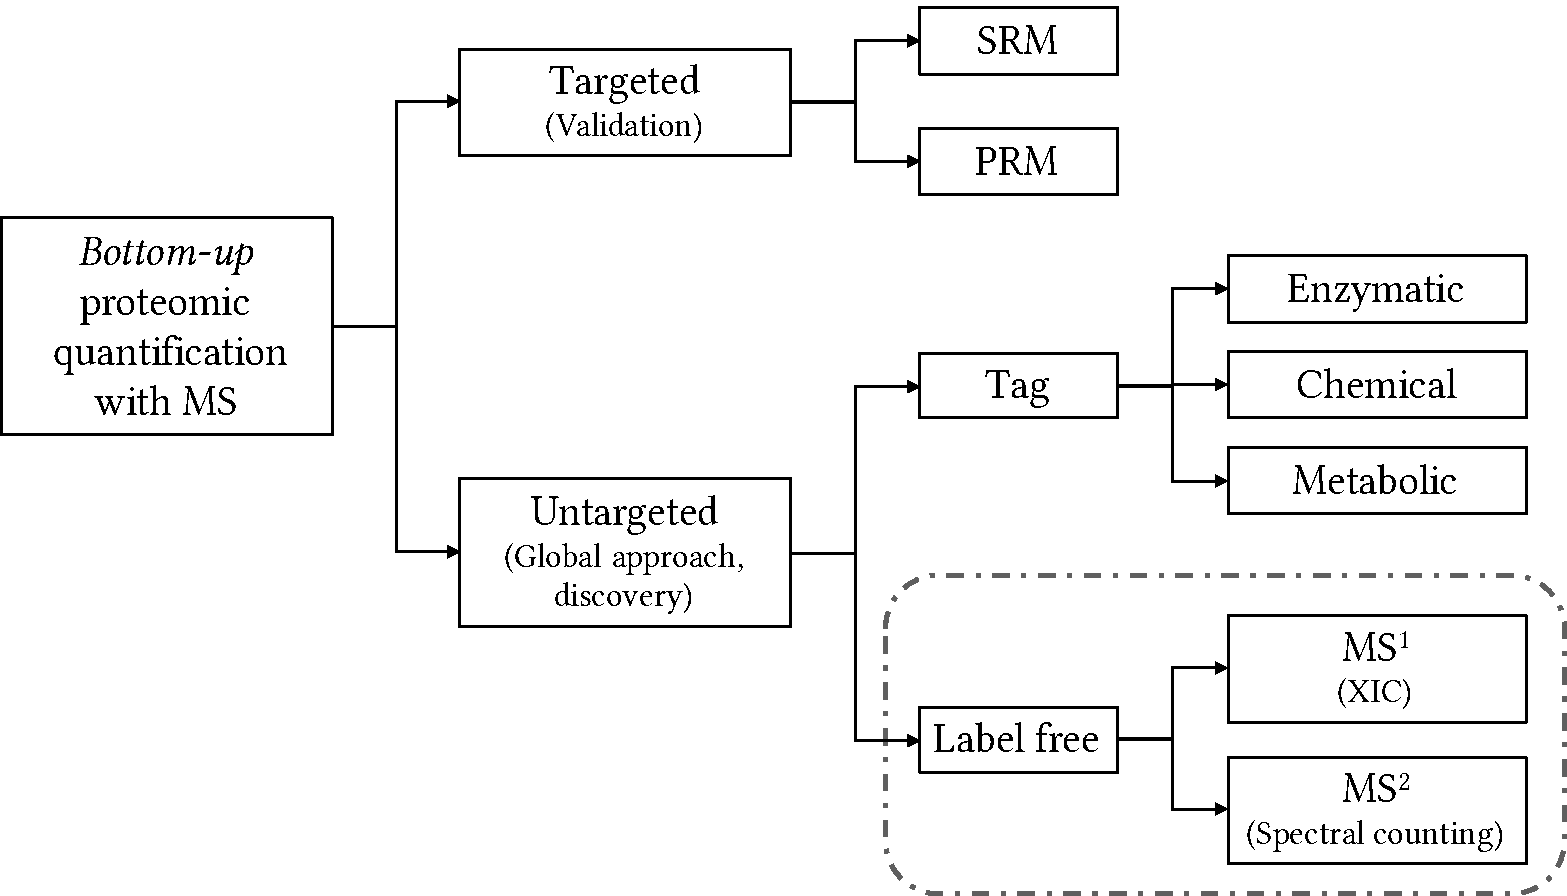
\includegraphics[scale=0.56]{background/MSproteomicsQuant.pdf}\centering
    \caption[Bottom-up quantification approaches]{\label{fig:msbottomupQuant}%
    \textbf{Bottom-up quantification approaches}.
    The work presented in this thesis relies on proteomic data
    that has been acquired through a \gls{DDA} bottom-up label-free
    \gls{MS/MS} approach (dashed frame).
    }
\end{figure}

Untargeted strategies provide only relative quantification
but are the most suitable for global approaches or discovery projects.
\emph{Tag} methods are favoured
when the study interest is about the differential expression of proteomes between
different conditions.
\emph{Label-free} ones are the most suitable for obtaining an overview of
the proteome landscape of disparate samples.
They are also the fastest and simplest approach to set up,
and thus, are favoured in studies where the number of samples is important.\mybr\

Tag strategies~\mycite{Zhou2014-vp} label the proteins (before or after extraction)
with stable isotopes (see \Cref{tab:isotope}).
For each condition, a specific isotope is used.
Thus, the proteins and peptides
have exactly identical physicochemical properties,
have the same behaviour through the protocols, and
only their mass can differentiate them.
The labelling can be either
enzymatic (\eg\ \isotope[18]{O}-labelling~\mycite{Ye2009-st}),
chemical (\eg\ \glsentrydesc{ICAT} (\gls{ICAT})~\mycite{Gygi1999-pe},
\glsentrydesc{iTRAQ} (\gls{iTRAQ})~\mycite{Ross2004-bn},
\glsentrydesc{TMT} (\gls{TMT})~\mycite{Thompson2003-we},
dimethyl labelling~\mycite{Hsu2003-aj},
or \glsentrydesc{2D-DIGE} (\gls{2D-DIGE})~\mycite{Unlu1997-vn}),
or metabolic (\eg\ \glsentrydesc{SILAC} (\gls{SILAC})~\mycite{Chen2015-zp}).
Some tag approaches have multiplexing protocols.\mybr\

\emph{Label-free} strategies~\mycite{Hsu2003-aj,Neilson2011-gi,Sandin2014-ow}
analyse the proteins after their digestion with the trypsin.
Since there is any marking in these methods, multiplexing is impossible.
Two different methods can quantify the relative abundance of the proteins.
\glsentrydesc{XIC} (\gls{XIC})~\mycite{Higgs2013-jm}
which quantifies each peptide by extracting its ion currents,
its molecular mass and retention time (MS1) (or the ones of its fragments (MS2)),
and then by integrating the area under the curve (\gls{AUC}) of the peptide
monoisotopic molecular mass (p),
and the following isotopic molecular mass peaks (p+1) and (p+2).
The \gls{XIC} assumption is that more concentrated is the peptide and
greater the \gls{AUC} is.
Spectral counting (also called MS2 quantification)
quantifies proteins based on the assumption that
the more abundant a protein is, the more this protein is selected to be fragmented;
thus the total number of \gls{MS/MS} spectra that can be mapped back to
the protein can be used to estimate it.
Unfortunately, this technique is lacking accuracy for the low detected proteins
compared to the others.\mybr\

Note that since there are many possible \ms\ approaches~\mycite{Bantscheff2012-ms},
in the following section, I focus on the one
that initially generated the proteomic datasets
I am reusing for this thesis (see \Cref{sec:ProteoData}).
Thus, I describe one widespread \emph{bottom-up} approach,
\ie\ the label-free \gls{LC-MS/MS} protocol
(also known as \emph{shotgun proteomics})~\mycite{Cox2011,Zhang2013}.
The following segments may be suitable for other methods as well.\mybr\

\subsection{Sample preparation}\label{subsec:ProtSampPrep}
Protocols to prepare samples for proteome analyses are generally much simpler
than the ones for \Rnaseq.
However, as proteins are also more complex and heterogeneous
than \DNA\ and \RNA~\mycite{Bruce2013}, there is a broader choice of them
in order to adapt to any requirement~\mycite{Feist2015}.\mybr\

\subsubsection{Sample collection and conservation}
\minisec{Collection}
\citet{Feist2015} report that traditional dissection, biopsies, blood draws and
other methods can deliver adequate samples for proteome analysis.\mybr\

\minisec{Conservation}
Recent developments have significantly improved proteome analysis from
formalin-fixed paraffin-embedded (\gls{FFPE}) samples \mycite{Steiner2014}.
As they are still evolving,
they may compare soon to fresh-frozen (\gls{FF}) samples.
However, for now, fresh or \gls{FF} samples are remaining the best primary sources.\mybr\

\subsubsection{Protein extraction and contaminant removal}
\minisec{Protein extraction}
Contrariwise to the collection step, \citet{Feist2015} explain that the crucial
consideration is the cell lysis and the extraction approaches used on
the protein as they may interact and disrupt the later characterisation step and
thus require appropriate picking. Besides, the physicochemical properties of
the proteins are far more heterogeneous than for \DNA\ or \RNA\ molecules~\mycite{Bruce2013}
and may be incompatible with many extraction protocols.\mybr\

\minisec{Contaminant removal}
\citet{Gutstein2008,Bodzon-Kulakowska2007,Visser2005,Hilbrig2003} review various
examples of mechanical and chemical extraction and contaminant removal methods.
Indeed, contaminants and detergents require to be eliminated from the samples
before analysis as, in the typical \gls{Bottom-up} approach, they interfere
with the digestion, the separation and fragmentations steps; precipitation and
filtering (based on molecular weight cut-off) strategies are the best in the
context of \gls{Bottom-up} \ms\ analysis~\mycite{Feist2015}. Indeed, many
extraction solvents are inappropriate for \ms. Precipitations may denature the
proteins, but this is usually irrelevant in this situation.
\citet{Feist2015} review different precipitation protocols
and emphasise that caution is needed
for the next re-suspension step to avoid missing a substantial part of the
sample proteome. They list several techniques and approaches in this regard.\mybr\

\subsection{\enquote{Simplification} of the samples}\label{subsec:simpleProt}

High-throughput bottom-up workflows (including \gls{LC-MS/MS}) generally
aim to decrease the sample complexity to analyse while increasing the depth
of proteomic coverage~\mycite{Zhang2014,Bruce2013,Cox2011}. Indeed,
many aspects may impede the characterisation of the proteins.
For example, the broad physicochemical scope of the proteins will
require various protocols to be handled efficiently.
Their concentrations in a sample may saturate the \ms\ characterisation capacity
as the very abundant proteins are easily detected and quantified while rarer
proteins may be missed entirely without specific precautions~\mycite{Liu2009,%
Cappadona2012} or without unbearably increasing the
analysis time per sample~\mycite{Nilsson2010}.
On the other hand, strategies to decrease saturation effects can also be used
instead~\mycite{Zhang2014}.\mybr\

Hence, the usual workflow will usually involve the denaturation, the reducing,
the alkylation and the digestion of the proteins. The peptide mixture products
are then separated in smaller fractions before subjection to \ms\ so to increase
the coverage depth
while keeping a reasonable analysis time-frame~\mycite{Aebersold2003,Cox2011,Zhang2013}.
\Cref{fig:proteomics} presents a general overview of one possible workflow.
Indeed, the various \emph{simplification} steps may happen in a different order
than I report hereinafter; they may also happen concomitantly. Additionally,
protocols may skip or inversely involve several times the same type of
simplification step. For example, protocols may present
\emph{proteins} fractioning as the first step
and then \emph{peptides} fractioning as a later one.\mybr\

\begin{figure}[!htb]
    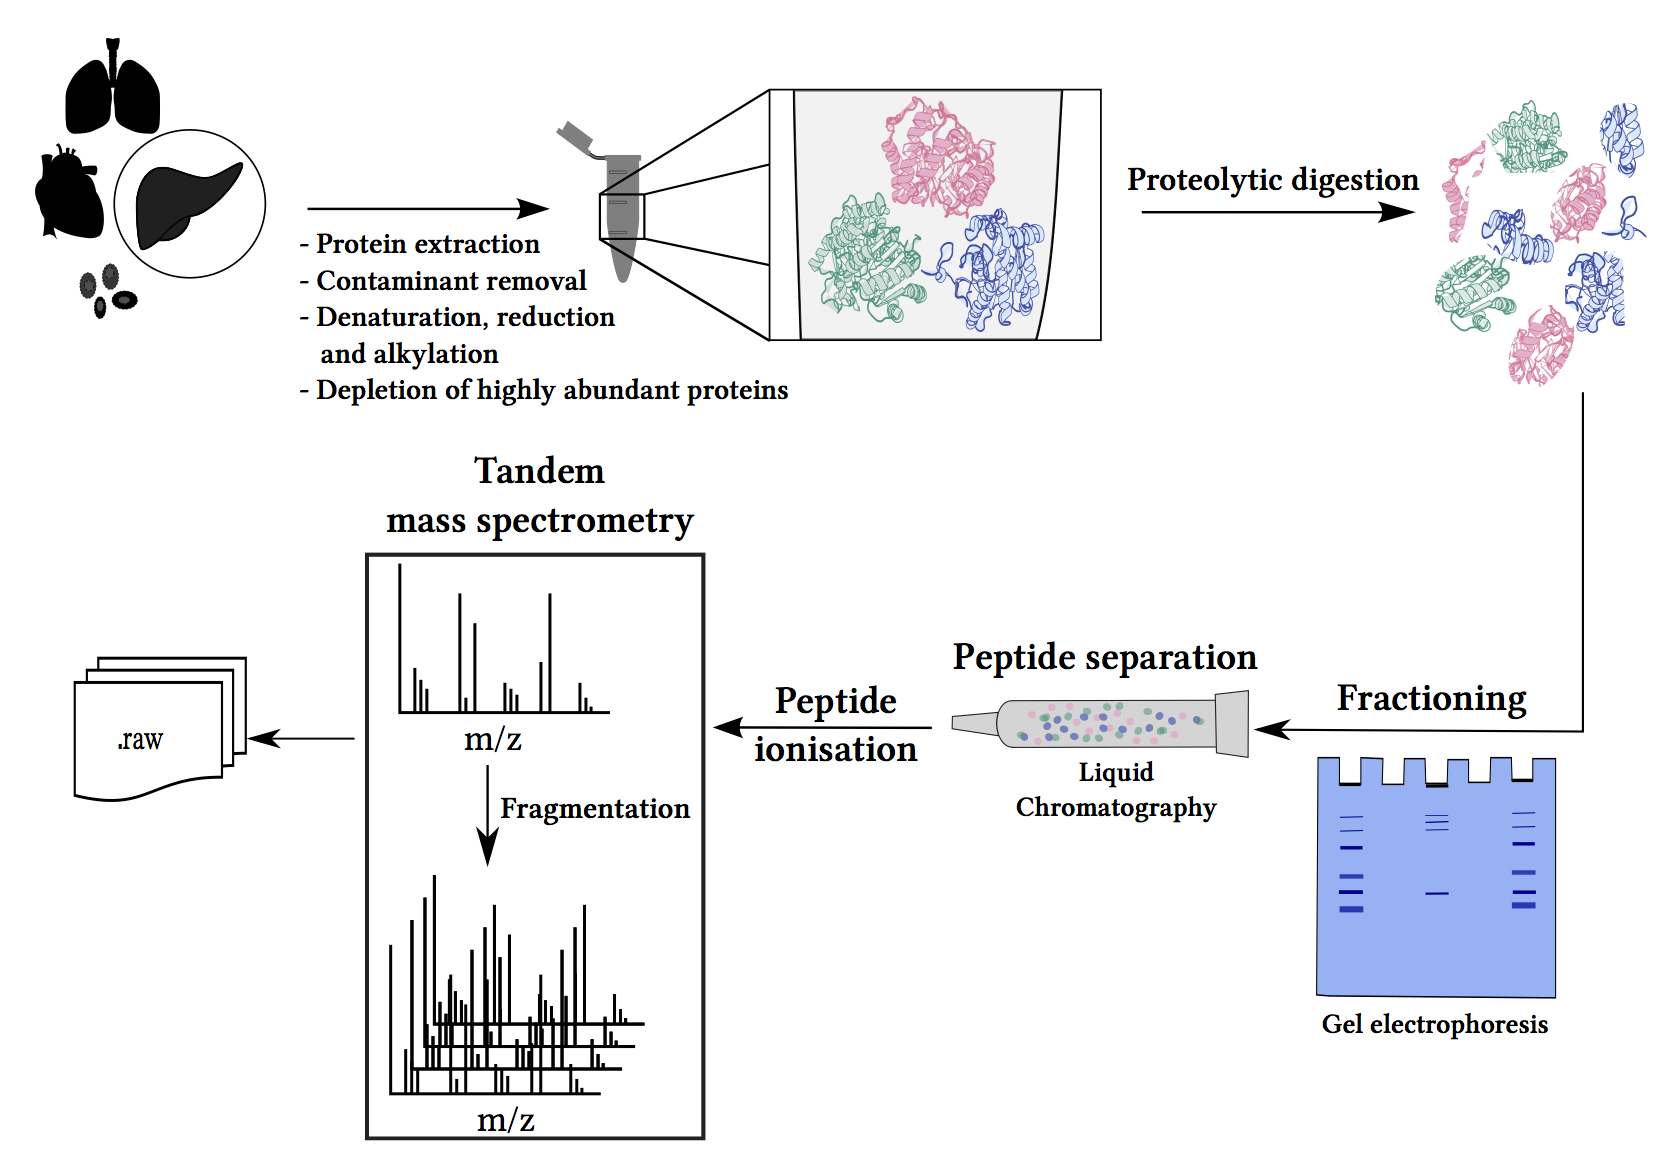
\includegraphics[scale=0.65]{background/proteomicWorkflow.png}\centering
    \caption[Overview of proteomic data generation]{\label{fig:proteomics}%
    \textbf{Overview of proteomic data generation}.}
\end{figure}

\subsubsection{Denaturation, Reduction and alkylation}

These steps may happen simultaneously to other steps. For example, they may
occur during the extraction, the depletion or the digestion. They help to protect
the proteins from endogenous proteases and separate the protein complexes. They
also help the relative linearisation of the proteins and, to some extent,
the homogenisation of the crude mixtures~\mycite{Feist2015,Bruce2013}.\mybr\

\subsubsection{Depletion of highly abundant proteins}

Regrettably, the proteomic field lacks amplification methods, and
there are very few strategies to remove the highly abundant proteins. Fortunately,
these are very limited in number and can be precisely targeted.
\citet{Zhang2014} report two useful strategies. The first one aims to remove
them entirely from the sample, either by selective
precipitation or by (more expensive) specific antibody-arrays.
The second approach aims to the equalisation of the proteome.
It may be based either on combinatorial ligand libraries involving
bead-supported ligands (on a similar model to \Rnaseq\ protocols)
or on specific protease mixtures\footnote{The former method uses bead-conjugated
hexapeptide ligands to capture (approximatively) equimolar amounts of proteins.
The very abundant proteins will bind till saturation to the beads, and their
remaining part in solution is washed off. This cheaper method has drawbacks.
For example, it presupposes that every protein has a corresponding ligand to bind.
\\\citet{MichaelMentenDepletion}, for example, describes the latter method. The
key to this protocol is to digest the most abundant proteins in peptides while
keeping the bulk of the other proteins intact.
Then, the peptides are removed by filtering their molecular size.}.\mybr\

In general, the equalisation of the proteome improves the characterisation
of the scarcer proteins~\mycite{Zhang2014} while they may introduce skewness
to the analyses (due to the relative protein proportions).\mybr\

\subsubsection{Proteolytic digestion}
It may seem contradictory to digest the proteins into peptide mixtures as a means
of \emph{simplification}. Nevertheless, while the main drawback is the inability
to distinguish between proteoforms~\mycite{Bruce2013}, it improves the proteins
characterisation on several points.\mybr\
\begin{itemize}
    \item It helps to homogenise the sample: peptides present closer
        physicochemical properties to each other than proteins~\mycite{Zhang2014}.
        Also, peptide separations (by gel or \gls{LC}) are easier than
        for proteins (see \Cref{subsub:sepMethods}).
    \item \ms\ is also more sensitive to the peptides than to the proteins
        due to being more sensitive towards lower molecular-weight molecules~%
        \mycite{Vitek2009,Cox2011}. Proteins may also be too large to be
        fragmented (\eg\ with \gls{CID})~\mycite{Bruce2013}.
    \item It is also easier to accurately characterise (identification and
        quantification) smaller molecules. Large proteins with similar
        compositions present very similar molecular mass and may be impossible
        to discriminate. On the other hand, the sequence-specific enzymatic
        digestion gives hints on the protein sequence.
    \item Finally, it increases the coverage of the less abundant proteins~\mycite{Zhang2014}.
        Indeed, each protein is represented by multiple
        peptides hence increasing the sampling probability. Often, one or a small
        number of \gls{LC-MS/MS}-characterised peptides is enough to identify the
        parent protein~\mycite{Bruce2013}.
        Furthermore, as mentioned previously, well-designed digestion can deplete
        the final mixture of abundant proteins.
\end{itemize}

The digestion may happen in-gel or in-solution. Both are very well-used.
In-gel digestion is very common in bottom-up approaches based on \gls{LC-MS/MS}
as it also provides directly the fractioning and it deals better with the more
complex samples. Often, the gel will contain, in addition to the protease, a few
chemical reagents that handle other steps (\eg\ chaotropic reagents to denature
the proteins at the same time). However, it requires greater time and amount of
starting material than for the in-solution digestion. In-solution digestion,
on the other hand, is the simplest and the most popular
digestion approach among all the proteome studies in general. It usually
precedes filtering and fractioning steps. More recently, a hybrid method
combining both methods has been developed and
named \acrfull{FASP}~\mycite{Manza2005,Wisniewski2009}.\mybr\

Although there are other enzymes for restrictive digestion,
trypsin is the gold standard protease~\mycite{Zhang2014}.
It cuts very specifically after arginine (R) or lysine (K) \glspl{aa}.
Circularity also explains trypsin's popularity:
as more studies are using it, more data are available for comparison;
hence more studies use it.\mybr\

\subsubsection{Separation methods (fractioning)}\label{subsub:sepMethods}
Fractioning is the principal method to simplify sample complexity. It also allows
focusing selectively on subcellular fractions when needed. Indeed, one may want
to study in particular organelles, cell compartments or other kinds of the proteome
(\eg\ phosphorylated or glycosylated proteins)~\mycite{Cox2011}. Besides,
fractioning is also a good strategy to reduce the impact of undersampling and
increase repeatability between analyses.
With \gls{MS} being prone to undersampling,
repeated analyses may lack yielding the same
protein identifications,
as different sets of peptides may get sampled.\mybr\

Several methods may fraction peptide mixture. Protocols may involve many of their
various combinations. However, the sequential use of a gel and \gls{LC} is
the most common for unknown complex peptides (or proteins) mixtures before
\ms\ analyses.\mybr\

\minisec{Precipitation}
They are very easy to perform, and they usually involve solvent gradients. While
their use is frequent for desalting crude mixtures, it is also quite limited
for protein mixtures as other separation methods (based either on gel or
capillarity such as \gls{LC}), are more performant.\mybr\

\minisec{Gel electrophoresis based separation}
Many protocols involve a first gel-based separation method before the
liquid-based separation and fragmentation of\enspace\gls{LC-MS/MS}~\mycite{Feist2015}.\mybr\

The gel separation may comprise one step or two, which are respectively named
one-dimension (1D) and two-dimensions (2D) gels.\mybr\

The general sample preparation for bottom-up proteomics is a 1D-gel approach.
It comprehends a denaturing alkylating gel (usually \gls{SDS-PAGE} but others are
possible, \eg\ \gls{LDS-PAGE})~\mycite{Shevchenko2006}. Thus, the proteins lose
all their quaternary, tertiary and secondary structures. The separation relies
then on the length of the proteins. Indeed, \gls{SDS} molecules carry negative
charges, and they bind to the proteins proportionally to their length, and as an
electric field is applied to the gel, the proteins migrate towards the positive
side of the gel at different speeds due to their difference in their mass-charge
ratio. As the 1D protocol is faster than the 2D one, its use is more common. The latter is
usually more selective as it relies on very similar principles but in two separate
steps\footnote{Usually, the proteins are first separated based on their
isoelectric point in a \emph{native} gel (as opposed to a denaturing one).
An \gls{ampholyte} reagent is added to the gel which ensures a stable
gradient of \gls{pH} through the gel. The proteins migrate until they reached a
\gls{pH} region where their overall charge is neutral. In a second time, the
proteins are separated perpendicularly this time on their mass after the addition
of \gls{SDS} or an alike reagent.}.\mybr\

Note that when the gel contains a protease, it separates peptides instead.\mybr\

\minisec{Liquid chromatography (LC)}

\vspace{-0.5mm}
Chromatography is a technique of choice for the separation of mixtures into their
components or --- at least --- in simpler mixtures. \gls{LC}, as any
chromatography, involves a \emph{mobile} and a \emph{stationary} phase.
The mobile phase comprises an eluent (\ie\ a solvent) and the mixture to be
separated. A column plays the stationary phase part.
High pressure may be applied (\eg\ \glsxtrfull{HPLC} or \glsxtrfull{UPLC})
to accelerate the process.\mybr\

\vspace{-0.5mm}
The separation relies on the difference of affinity of the mixture components
between the mobile and stationary phases. Many combinations are possible. However,
any poor choice may precipitate the mixture on the (\emph{extremely})
expensive column which means that both the column and the mixture will be lost.
Hence, in discovery mode and for complex mixtures (as for proteins extracts),
instead of using a \emph{normal phase}, \ie\ crude silica-gel, column (which
interacts tightly with polar molecules such as peptides and may prevent them to
interact with the mobile phase afterwards), a \emph{reversed phase} column
is more common. In these columns, the silica-gel is modified and has been
attached to long hydrocarbon chain. Thus, the column is unable to fix anything
permanently. Along with a \gls{RPLC} column, polar eluants are used. These
interact strongly with charged proteins and peptides. Hence, the separation
occurs on the polarity of the molecules and the most hydrophobic a molecule,
the longest it will remain in the column as it will present fewer interactions
with the eluent.\mybr\

\vspace{-0.5mm}
The ease of coupling this powerful method to the (also powerful) \ms\ explains
why \gls{LC-MS} is so widespread today. Their combined use also allows high
repeatability and optimised running time.\mybr\
\vspace{-1mm}

\subsection{Characterisation through Fragmentation profiles}
\vspace{-3mm}

The first reported use of the principle underlying \ms\ happened in 1913 when
Sir Joseph John Thomson channelled a stream of neon ions through an electromagnetic
field and captured its deflection on a photographic plate~\mycite{Thomson1913}.
Arthur Dempster and Francis W. Aston created the first mass spectrometers in 1918
and 1919 respectively~\mycite{Aston1919}.
%Arthur Dempster built a first mass spectrometer in 1918. Francis  William
%Aston (Thomson's student) created his complete one in 1919~\mycite{Aston1919}.
\begin{comment}
\ms\ became rapidly a pillar
of the so-called \emph{modern analytical techniques} in Chemistry as it allows
for a large spectrum of molecules of interest, the detection,
the characterisation and even, for the smaller ones, the resolution of their
structures.
\end{comment}
In this context, the use of \ms\ is quite recent in proteomics
as it has been developing from the 1980s onwards~\mycite{BiomolBio}.\mybr\

\subsubsection{General principle}

\ms\ relays on the following principle: molecules of interest are ionised
into charged particles then the mass analyser separates them in the gas phase
based on their total mass $(m)$ to charge $(z)$ ratio, \ie\ $m/z$.
A detector collects all these ions and translates their signal (intensity versus
$m/z$) to an electric one which is the output serving as raw data for the
later analyses. In the simpler case, the molecules are singly charged ($z=1$),
and only their molecular mass is recorded. However, it is quite common for the
molecules to carry more than one electric charge and that if the energy used for
the ionisation is substantial, they may also forego fragmentation and internal
reactions that will result to the production of many spectra. The collection
of spectra obtained from a single peptide ultimately increases the accuracy of
the mass measurement and the identification of the peptide~\mycite{BiomolBio}.
Indeed, these peptide-mass profiles are a very effective way to identify
proteins in very short lapses of time as long a reference database is available
for the studied organism~\mycite{Pappin1993}. The recent completion of the human
genome sequence and many other organisms has accelerated the general use of this
analytical method~\mycite{Luge2016}. Besides, recent developments have
shown that the use of two mass spectrometers in tandem (\gls{MS/MS}) reduces
the number of missed proteins significantly while keeping reasonable running
times and it is more potent than excessive fractioning as is the improvement
of \gls{HPLC}~\mycite{Cox2011}.\mybr\

\subsubsection{Ionisation}

While there are other methods (more adapted to small organic molecules)
two \emph{soft} ionisation methods are routinely used for proteomic samples:
\acrfull{MALDI} and \acrfull{ESI}.\mybr\

\gls{MALDI} is very useful for large molecules. It allows creating ions with a
minimum of fragmentation (if any at all). The molecules are fixed onto a matrix
(a gel) and then a pulsed \gls{laser} irradiates the sample which provokes the
ablation and then the desorption from the matrix and ionisation of the molecules.
This method had increased popularity as separation gels (\eg\ \gls{SDS-PAGE})
may be used directly for both steps. \mycite{BiomolBio}.
However, it requires compatible mass spectrometers
with this ionisation technique~\mycite{Zhang2014,Walther2010}.\mybr\

\gls{ESI} is currently the most popular technique of ionisation, mainly
because it may be used with a large panel of different analysers and that it
interfaces efficiently with \gls{HPLC} or \gls{UPLC}. An electrostatic method
performs the ionisation. The application of a high electric potential on
a needle through which a liquid (containing the dissolved analyte peptides)
is passing provokes its dispersion into small and highly charged droplets.
These droplets start to evaporate to the point where the charge on their surface
is so high that the desorption of the analytes occurs.  The analytes are then
in an ionised form (often many charges). They are then released into the mass
spectrometer. \mycite{Walther2010}\mybr\

\subsubsection{Mass analyser}

Many different mass analyser designs are available. They all share two properties:
they accelerate the ions (in a vacuum), so all the ions share the same kinetic
energy, and then they deflect (and thus resolve) the ions based on
their various $m/z$. Many are also
capable of trapping and storing specific ranges of ions for more in-depth analyses until
they release them based on their $m/z$.
The most common commercial analysers include quadrupole (Q), \acrfull{LIT},
\acrfull{TOF}, ion traps and most recent \gls{FT} analysers such as \acrfull{ICR}
and \orbi.
The choice of one analyser over others or any combination of them
depends on many factors (including availability).~\mycite{Haag2016}\mybr\

In \Cref{sec:appMassAnalysers},
I review the analysers involved in
the production of the raw proteomic data used in this thesis.
Indeed, all the datasets have been
produced by a combination of \acrfull{LTQ} and \orbi.% I also review very
%shortly the quadrupole analyser. (See~\citet{Haag2016} for more details on other
%types of analysers.)
\mybr\
\begin{comment}
\minisec{Quadrupole analyser}

It is one of the most popular analysers. In fact, they are cheap compared to the
others. They are also compact, durable and reliable. The quadrupole analyser can
filter the ions based on their difference of $m/z$. They are adequately
named quadrupole as they comprise four cylindrical or hyperbolic rods in
parallel to each other. Opposite rods are connected together electrically and
\gls{RF} potential is applied. A \gls{DC} potential is superimposed on the
\gls{RF} one. These combinations of \gls{RF} and \gls{DC} potentials constrain the
ions to oscillate between the rods as they pass through them. Hence, by tuning
the \gls{RF} and \gls{DC}, it is easy to select for which range of $m/z$ ions
will have a stable trajectory and thus the only one detected. Indeed, the
ions with unstable trajectory will collide with the rods and be \enquote{filtered}
out. If used in \enquote{\gls{RF}-only} mode (\gls{DC} reduced to a minimum),
the quadrupole may have other applications. For example, it can guide specific
$m/z$ ions to other areas (while the bulk of ions will remain trapped).
It may also be used as collision cells for \gls{CID}: by introducing an inert
gas and tuning with the \gls{RF}-energy, the amount of fragmentation undergone
by the targeted ions can be precisely controlled. \mycite{Haag2016}\\
The quadrupole analyser is also qualified as the \emph{mass filter}.\mybr\

\minisec{\Acrfull{LTQ}}
\gls{LTQ} is a particular kind of \acrfull{LIT} which is in principle a sort of
a quadrupole mass analyser~\mycite{Zhang2014}. A \gls{LTQ} uses a set of
quadrupole rods and a two-dimensional \gls{RF} field confines the ions radially.
Besides, a static electrical potential is applied to end electrodes which
forbid the ions to escape axially. However, the quadrupole is commonly segmented
into three parts which ensure a perfect homogeneity of the electric field of the
trap area and thus avoiding ion loss when the trapping is done.
While they may be used as an ion trap, they
may be also used as a simple mass filter. \gls{RF} voltage is tuned to produce
multi-frequency resonance ejection waveforms are applied as to
eliminate all the undesirable ions in the trap before the fragmentation and mass
analysis of the remaining ones. Frequently, these \glspl{LTQ} are used as a
front-end to other mass analysers as they have high injection efficiencies and
high ion storage capacities. They may be equipped then with two biased radial
ejection slits and then be used with two detectors hence the signal-to-noise
ratio may be doubled.\mybr\

Compared with other traps, linear ion traps provide an enhanced dynamic range
with a reduced low mass cut-off as the ion cloud is
spatially distributed on a linear axis and not a 3D centre which improves the
sensitivity. And then, for example, the ions may then be accumulated before
being released into another mass analyser~\mycite{Madalinski2008}.\mybr\

\minisec{\orbi}
It is a very recent analyser and it relies on \gls{FT}. Recently,
there is increasing use of \glspl{FTMS} for proteomic studies. Indeed, these
\glspl{FTMS} are more precise than previous analysers and allow the detection of
a greater range of ions in very short lapses of time~\mycite{Scigelova2011}.
In this kind of analyser, ions are trapped and both orbit around and oscillate
in an electrostatic field between an inner and outer part of a central electrode
shaped as a spindle.
The ions can only move following the spindle long axis~\mycite{Makarov2000}.
While moving around the spindle the ions create a current.
The outer part of the spindle records images of this current.
Fourier transformation of these images allows obtaining very highly accurate
and sensitive mass spectra for a greater dynamic range than most of the
other analysers.~\mycite{Hu2005}\mybr\

\minisec{\gls{LTQ}-\orbi}
It is a hybrid (tandem) mass spectrometer that uses \gls{ESI} for the ionisation
step and has an \gls{LTQ} as a first analyser (MS$^1$)
and an \orbi\ as a second one (MS$^2$).
This \gls{MS/MS} enables multiple levels of
fragmentation for the elucidation of a wide range of peptides and can be coupled
with an \gls{ESI} which is a continuous source of ionisation. This instrument
allows analysing proteomic samples optimally both in terms of starting material,
time~\mycite{Scigelova2011} and provides \enquote{ultrahigh} mass resolution,
high mass accuracy
and enhanced dynamic range with respect to mass accuracy~\mycite{Madalinski2008}.\mybr\
\end{comment}

\subsubsection{Fragmentation techniques~\mycite{Zhang2014}}

The overall quality and success of peptide (and then proteins)
identification depends largely on the quality of ion fragmentation.
Tandem-\gls{MS} (\gls{MS/MS}) improves the identification of the peptides
by cleverly increasing the number of fragmentations.
Indeed, the first \ms\ is
used to select specific ions (hence known $m/z$) to pass to a second \ms.
Thus for each \emph{precursor} ion, a collection of fragmentation mass spectra
can be gathered. The peptide sequences are then more likely to be accurate, and
the risk of false positive is significantly decreased.\mybr\

While the experimenter may want to limit fragmentation,
they may also often use devoted techniques to increase it.
There are schematically three different classes of fragmentation techniques:
collisional, electron-based or photon-based.
The collisional category, \gls{CID} (see \Cref{sec:appMassAnalysers}),
is widespread.
The chosen ion is introduced in the collision cell,
and its collusion with an inert gas particle produces kinetic energy,
which transforms into internal energy.
The fragmentation happens when this internal energy is sufficient to activate
the dissociation of the ion.
Another related and slightly more effective method
for higher charge state ions is the \acrfull{HCD}.
This latest method (developed by ThermoFisher for \orbi\ analysers),
has gained popularity with the development of quantitative proteomics
(\eg\ \gls{iTRAQ})
as it provides in parallel peptide identification and quantitation.
In the electron-based category,
the most common is probably the \acrfull{ETD} technique:
an anion donates an electron to a cationic peptide,
and this transfer initiates
the fragmentation of the peptide backbone~\mycite{Syka2004}.
For the other categories,
see the review from \citet{Zhang2014} and the included literature.\mybr\

\subsubsection{Acquisition modes}
There are two possible acquisition modes: \gls{DDA} and \gls{DIA}.\mybr\

The most common \gls{DDA} approach has many advantages~\mycite{AebersoldMann2016}.
It is unbiased and free from any hypothesis,
and hence a great tool for global discovery study.
It surveys the proteome all at once,
and prior knowledge is unrequired.
Its popularity increased concomitantly to the increased availability of
high-quality genome and gene sequence databases
and more recent technical advances in \ms\
(development of new protein/peptide ionisation
and fragmentation methods)~\mycite{Aebersold2003,Cox2011,Zhang2014}.
The main \gls{DDA} limitation~\mycite{Guillaumot2017-ba} is its inability
to select all the existing peptidic ions for fragmentation by \gls{MS/MS}.
The stochastic selection is biased by
each peptide ionisation efficiency
and the possible peptides coelution
while the \gls{LC} before being introduced in the \ms.
In practice, the instrument first scans quickly the current eluting peptides (MS1)
before a few (the ``top N'') precursors are selected
one after the other for fragmentation (MS2).
One MS1 spectrum with N MS2 spectra constitute one duty cycle,
which usually lasts about 1s.
Peptides elute over 30 to 40s,
and software tools that drive the instruments can predict peptidic peaks
and thus will increase the chance of high-quality MS2 spectra
by selecting the peptides at their maximum abundance.
A dynamic exclusion window avoids the same peptides to be repeatedly selected and
new targets to be fragmented.
MS1 spectra allow selecting potential peptides to fragment and their intensity.
MS2 spectra are used to identify the peptides later.\mybr\

\gls{DIA} approaches are more complicated
as no precursor is selected and
all the coeluted peptides are fragmented at the same time.
The sustained interest in \gls{DIA} methods is because
they provide a fuller overview of the proteomes.
They can generate comprehensive fragment-ion maps for
specific proteoforms~\mycite{Chapman2014}.
Often \gls{DIA} is performed after a short \gls{DDA} survey
that establishes a small reference spectrum library
to help with the analyse of the MS2 spectra.
In the past decade, \gls{DIA} studies number has expanded,
particularly with methods such as SWATH-\ms~\mycite{Gillet2012-ce}
(for proteome quantification).
\gls{DIA} methods are likely to gain even more popularity
as many efforts are put into their developments~\mycite{Hu2016-ri}.\mybr\

\subsection{Bioinformatic strategies for proteomics studies}\label{sec:bioinfProt}

\ms-based proteomics is quite challenging,
and the major bottleneck of proteomics pipelines remains
the data analysis~\mycite{Chen2016,perseus2016}.
Since mass spectrometers' raw data output
for proteomics is directly uninterpretable by a human,
it needs processing before being meaningful.
Because the sheer amount of produced data is in the terabyte (\gls{TB}) range,
it prohibits any manual handling and requires automation~\mycite{Codrea2016},
most notably for the data matching (\ms\ spectra to databases content) and
protein identification steps~\mycite{Nilsson2010}.\mybr\

The protein identification process leads to three computational challenges:
peptide identification, protein inference and result validation~\mycite{Huang2012-nr}.
Besides, shotgun proteomics produce highly redundant data:
peptide subsets that ionise better than the rest
are repeatedly and preferentially selected for fragmentation
and thus will produce more \gls{MS/MS} spectra~\mycite{Eriksson2007-si,Koziol2013-si}.
On the other hand,
subsets of peptides are undetectable with the currently available technology;
they hardly ionise, or have a weak signal that is masked
by other more abundant or more ionisable peptides.
Thus, shotgun experiments are plagued by missing data~\mycite{Stead2008-in,Lazar2016-oe}.\mybr\

As for \Rnaseq, for each proteomics analysis step,
there are many tools.
Many integrate a few (if not all) of the steps described in the following pages,
\eg\ \softFoCi{MaxQuant}{http://www.maxquant.org}{maxquant2016}
or \softFoCi{OpenMS}{http://www.openms.de/}{Pfeuffer2017-dh}.
From the raw data acquisition to downstream analyses
(or any of the intermediate steps),
pipelines integrate many different combinations of tools~\mycite{Vitek2009}.\mybr\

The pipelines vary depending on experimental design, data type
(\ie\ expression, modification state or interactions map)
and the practical creation of the data (\eg\ method of separation,
mass analyser kind, acquisition mode).
Many of these factors are interconnected in \ms\
and while their individual effects have been extensively studied,
designing a sound pipeline may be overlooked easily~\mycite{LCMSflaws,Maes2016-xo}.
However,
this risk is reduced as
many tools imply working upstream or downstream with specific tools,
\eg\ the output of \soft{MaxQuant} (raw data to protein quantification) is
ready for use by \softFoCi{Perseus}{http://www.perseus-framework.org}{perseus2016}
(downstream analyses such pattern recognition,
time-series analysis, cross-omics comparisons and multiple hypothesis testing).
Besides, as files from mass spectrometers are usually encoded
in proprietary (commercial) formats,
there may be a limited choice of available tools or software
for a specific combination of analysis and data.
A few open file formats (and their appropriate converters) exist
(\eg\ \mzml\ format~\mycite{mzML}
and \href{http://proteowizard.sourceforge.net/}{\soft{ProteoWizard}}\footnote{%
\soft{ProteoWizard}: \href{http://proteowizard.sourceforge.net/}%
{http://proteowizard.sourceforge.net/}}~\mycite{proteowizard2012}),
however, they may lack recording a few critical points of the raw data,
and so, they may also be unfit for particular analyses.\mybr\

As bottom-up approaches are the most common,
their associated tools also tend to dominate
the \ms{}-based proteomic bioinformatics~\mycite{Lee2015-di}.
In the following pages,
I review the steps involved in the \gls{MS/MS} pipeline,
presented in \Cref{ch:datasets},
that has processed all the proteomic data presented in this thesis.\mybr\

\subsubsection{Signal processing and mass peaks detection}

The signal processing step comprises
the (noise) filtering (or \emph{denoising}),
the baseline correction (which eliminates systematic trends),
the signal normalisation (or \emph{centroiding}),
and the mass peaks detection~\mycite{Codrea2016,Nahnsen2013}.
These steps are highly automatised and
happens almost simultaneously to the signal acquisition.\mybr\

While mass peak picking may be done manually for smaller molecules,
the number of spectra in proteomic experiments
(in the order of 100,000 spectra for one sample)
require the automation of this task.
Even though instrument resolution has significantly improved over the last decade,
peaks can be smooth (\ie\ with a large signal-to-noise ratio (\gls{SNR}))
and easy to pick, or they can still be noisy
(\ie\ barely distinct from the background) and trickier to identify.
Peak width is related to the peptidic ion mass-to-charge ($m/z$),
the mass analyser resolution and acquisition parameters.
Algorithms may use this relation to detect peaks by
scanning the mass spectra for local maxima of expected widths. \mycite{Bauer2011}.
They can also rely on
the associated isotopic peak clusters of the molecular mass peak
(see \Cref{app:isotopes}).
These molecular peaks clusters (and their relative intensity) also provide
information that can resolve the atomic composition of the peptides~\mycite{Nitpick}.\mybr\

Optionally, a final molecular mass correction step can be applied to remove
modifications due to the ionisation process.\mybr\


\subsubsection{Peptide identification and validation}\label{subsub:peptideID}

An essential step of proteomic data processing is to identify and then validate
a peptide sequence for each molecular mass that has been detected.
Typically in \gls{LC-MS/MS},
the first \ms\ spectra (MS$^1$) are used for the estimation of the relative
quantification of each peptide,
while the fragmentation spectra (MS$^2$) give its identification~\mycite{Codrea2016}.
The higher the number of fragments to identify a peptide,
the more robust the identification is.\mybr\

\minisec{Matching spectra to peptide sequences}
There are three main possibilities for protein/peptide spectra matching.\mybr\
\begin{itemize}[topsep=0pt,nosep]
    \item Matching the experimental spectra to theoretical ones created by
        adequate \latin{in silico} digestion
        and fragmentation of proteins found in protein sequence databases such as
        UniProtKB/Swiss-Prot from \softFoCi{UniProt}{https://www.uniprot.org/}{UniProt2017},
        which is manually annotated and reviewed,
        UniProtKB/TrEMBL (automatically annotated, unreviewed), or
        from genomic sequence databases (\eg\ \softFo{NCBI}{https://www.ncbi.nlm.nih.gov/protein/})
        after \emph{\latin{in silico} translation} of the sequences.
        This type of matching requires database-dependent search engines,
        \eg\ \softFoCi{Mascot}{http://www.matrixscience.com/}{Perkins1999-yc}
        or \soft{Andromeda} from \soft{MaxQuant}.
    \item Matching the experimental spectra to other previous experimental spectra
        saved into a repository.
        This approach relies on spectral matching engines,
        \eg\ \softCi{HMMatch}{Wu2007-fu}.
    \item A \latin{de novo} \emph{sequencing} approach which consists of
        comparing the observed mass data to the theoretical mass
        of every possible peptide sequence.
        For example, see \softFoCi{PepNovo}{http://proteomics.ucsd.edu/Software/PepNovo/}{Frank2009-nb}.
\end{itemize}

The first two methods are favoured over \latin{de novo} peptide sequencing,
as the latter is very cumbersome and time-consuming.~\mycite{Codrea2016}
Note that there are also hybrid approaches based on \latin{de novo} sequencing and
database matching.\mybr\

Many search engines exist for matching \gls{MS/MS} spectra,
see \citet{Griss2016,Shteynberg2013,Eng2011} for reviews.
Furthermore\label{seg:moreAlgoisbetter},
combining the results of several search algorithms when possible improves
the final outcomes~\mycite{Sadygov2004-nl,Eng2011,Shteynberg2013,Griss2016}.\mybr\

Many algorithms (\eg\ \soft{SEQUEST} and \soft{Mascot}) rely on
the same information and parameters choices to match
(and score) the spectra to peptide sequences.\mybr\
\begin{itemize}[topsep=0pt,nosep]
    \item Fragmentation mode
    \item Digestion enzyme and the number of possible omitted cleavages
    \item Mass tolerance for $m/z$ ratio of peptidic and fragmented ions.
    \item Possible charges for the peptidic and fragmented ions.
    \item Knowledge database (the more a database is complete, accurate and adequate,
       the better and more robust is the peptide and protein identification).
\end{itemize}

\minisec{Scoring functions}

While algorithms assign \gls{MS/MS} spectra to peptide sequences,
they simultaneously compute a corresponding score
for each peptide-spectrum match (\psm).
This score summarises the quality of the assignment
and allows the selection of the best candidate-peptide for each spectrum.
Only the matches with the best \psm\ scores (if not the very best one only)
are reported and used in the next steps of the quantification process.\mybr\

\citet{Sadygov2004-nl} classify the scoring functions in four classes:
descriptive (\eg\ \softFoCi{SEQUEST}{http://fields.scripps.edu/yates/wp/}{Eng1994-eq})
interpretative, stochastic and probability-based modelling (\eg\ \soft{Mascot}).
While many of these functions return statistical scores
(\eg\ \soft{Mascot} and \soft{SEQUEST}),
many other return non-statistical ones.
For these latter ones,
tools such as \softFoCi{Percolator}{http://percolator.ms/}{Kall2007-qn,Spivak2009-zd}
or \softFoCi{PeptideProphet}{http://peptideprophet.sourceforge.net/}{Keller2002-dq,Ma2012-lu}
allow transforming their scores into probabilities,
and ease the application of threshold to remove unreliable matches~\mycite{Cottrell2011-gh}.
Regardless of whether the score is either statistical (including probability-based) or not,
searching the database to match spectra to peptide sequence is a statistical process.
Most \gls{MS/MS} spectra only partially cover a peptide sequence,
which leads to many ambiguities.
With the development of high-throughput \ms-based proteomics,
researchers dropped manual interpretation and validation
and moved towards empirical score thresholds~\mycite{Broshphd}.
Thresholds are a compromise between sensitivity and accuracy (or error rate),
\ie\ true positive (or correct) identifications proportion
\latin{versus} false positive (or incorrect) identifications proportion.
A high threshold for the scores reduces the error rate, but costs sensitively.
A low threshold accepts more \psms, but also more incorrect matches.\mybr\

In addition to the choice of threshold requiring an expert,
another complication is the unknown real error rate.
This situation led in the past in result discrepancies:
results based on the same data varied
as much as 50\% between different laboratories~\mycite{States2006-qb}.
It prompted journals to require validation
with standard statistical (comparable) measures,
and later the establishments of guidelines by the
community~\mycite{Bradshaw2006-dg,Binz2008-yz,Rodriguez2009-cc,Kinsinger2012-km}.\mybr\

\minisec{Peptide validation}

Today, among the many methods that validate the peptide assignment and
estimate its error rate,
the gold standard is the \gls{TDA}~\mycite{Perkins1999-yc,Elias2007-wi,Savitski2015-fx}.\mybr\

Many search engines compute a \pval\ for each of the \psms,
but it is insufficient to determine if multiple \psms\ are true matches.
A low p-value \psm\ has a low probability of being incorrect.
Because of the large number of \psms\ per experiment,
statistically, a portion of these \emph{are} incorrect.
Thus, other statistical measures
adjusting for multi-testing (see \Cref{multitesting})
are required.
Corrections (such as Bonferroni~\mycite{Shaffer1995-lp}) can be applied
though they are stringent and discard many correct \psms.
\glsentrydesc{FDR}~(\gls{FDR}) $[$\citet*{Benjamini1995-nf}$]$ is
estimates the proportion of incorrect \psms\
among all accepted \psms~\mycite{Nesvizhskii2010-mz,Aggarwal2015-hi},
see \Cref{eq:fdr-prot}.
Different approaches exist to estimate it.
The most favoured is \gls{TDA}
as it is non-parametric, easy to apply, and
it also has the advantage of working with non-statistical scores search engines.\mybr\

Instead of figuring out which the correct and incorrect \psms\ are,
the \glsentrydesc{TDA} (\gls{TDA}) aims to estimate
the overall \gls{FDR} associated with a specific collection of \psms.
In turn, this enables assessing the likelihood of each of the \psms\
in the collection~\mycite{Elias2007-wi}
(see following segments on \emph{q-values} and \gls{PEP}).
Besides, this approach can guide
the selection of sensitive \psm\ attributes
(\eg, elution time, charge, peptide length, score)
for filtering criteria to discern correct identifications~\mycite{Elias2010-kp}.
The critical elements of this method are
the creation of a \emph{decoy} database with sequences
that are incorrect but similar (while non-overlapping)
to the \emph{target} (\ie\ true) ones.
Consequently, any \psm\ found for a decoy sequence is by definition spurious.
The known proportion of decoy versus target sequences in the search space allows
the computation of the \gls{FDR}~\mycite{Elias2007-wi,Elias2010-kp}.\mybr\
\vspace{-9mm}

\begin{equation}\label{eq:fdr-prot}
    \tag{\gls{FDR}}
    \begin{split}
        {\text{FDR}} & =\frac{\text{Number of accepted \glspl{PSM}}_{\text{decoy}}}%
    {\text{Number of all accepted \glspl{PSM}}}\\
          & =\frac{\text{Number of accepted \glspl{PSM}}_{\text{decoy}}}%
    {\text{Number of accepted \glspl{PSM}}_{\text{decoy}}+\text{Number of accepted \glspl{PSM}}_{\text{target}}}
\end{split}
\raisetag{4\normalbaselineskip}
\end{equation}
\begin{comment}
\vspace{-6mm}
where:
{\small
\begin{itemize}[topsep=0pt,nosep]
    \item $\text{\emph{Number of accepted \glspl{PSM}}}_{\text{decoy}}$
is the number of \glspl{PSM} from decoy sequences
that are above a specified threshold $\mathcal{t}$,
    \item $\text{\emph{Number of all accepted \glspl{PSM}}}$
is the total number of accepted \glspl{PSM}
above the specified threshold $\mathcal{t}$,
including the accepted decoy \glspl{PSM}.
    \item $\text{\emph{Number of accepted \glspl{PSM}}}_{\text{target}}$
is the number of accepted \glspl{PSM} above the specified threshold $\mathcal{t}$.
\end{itemize}
}
\end{comment}

\vspace{-4mm}
For best effectiveness,
decoy and target peptide sequence databases are searched with the same parameters.
Furthermore, to ensure that
a wrong hit in the target database and a hit in the decoy one are as likely,
the decoy sequences have to be as similar as possible to the target ones
(concerning \gls{aa} frequencies and composition,
length, mass, charges, assigned scores).
There are different ways to design the decoy sequences.
For example, by reversing the peptide or protein sequences,
either with complete or pseudo-reversion (where the last \gls{aa} is kept in place).
Alternatively, by using stochastic methods on the target database
such as the randomisation of the sequences or
through the creation of new ones based on \glspl{aa} frequencies,
their length distribution,
and their number in the original database;
Markov chain models~\mycite{Gagniuc2017-nj} are often used
to mimic the closest target sequences.
Many studies explore and compare the different decoy creation
methods~\mycite{Elias2007-wi,Wang2009-ww,Elias2010-kp,Wright2016-as}.
As for the target database,
the decoy sequences are digested \latin{in silico} before the search.
While the search can be done independently
on the target and the decoy databases~\mycite{Blanco2009-u6},
\citet*{Elias2007-wi} report that
searching their resulting concatenation gives better results.\mybr\

Most of the search engines return multiple scores.
Hence, defining a proper threshold for each of them can be challenging or cumbersome.
A possible solution is \soft{Percolator},
which trains a \glsentrydesc{SVM} (\gls{SVM})~\mycite{Boser1992-yn}
to distinguish the correct and incorrect \psms{}~\mycite{Kall2007-qn}.
This machine learning based algorithm has several advantages.
It can exploit many scores and other specific data features
to automatically determine the best threshold
without overfitting to a particular collection of \psms.
Thus, comparisons of results between studies and laboratories are facilitated.
Moreover, many studies have reported that the use of \soft{Percolator}
improves the results in terms of both accuracy and sensitivity and
increases the overall number of identified peptides~\mycite{Granholm2014-cw,%
Xu2013-si,Tu2015-iy,The2016-dq,Wright2012-od}.
%Besides, many pipelines integrate it to provide
%the significance measures needed for publication.
\soft{Percolator} can either be used directly on
the collection of target and decoy \psms\
or as a post-processing step.\mybr\

\vspace{-0.7mm}
Algorithms inferring proteins identity also use
two other significance measures for \psm\ validation:
q-values and \gls{PEP}.\mybr\

\vspace{-0.7mm}
A possible definition of \psm's \emph{q-value}\label{qvalP} is
the minimal \gls{FDR} threshold for which the \psm\ is accepted as correct.
As the q-values are derived from the \gls{FDR},
which is specific to a \psm\ collection,
they are also (solely) specific to this collection.
For example,
\soft{Percolator} estimates the q-value
by using the score distribution from the \gls{TDA}.
On the other hand,
\glsentrydesc{PEP} (\gls{PEP})\label{PEP}
(also known as \emph{local \gls{FDR}}~\mycite{Efron2001-ai})
is the probability of a \psm\ being incorrect;
a \psm's \gls{PEP} is invariant regardless of the \psms\ collection.
A classical approach to estimating \glspl{PEP} uses
training sets of target and decoy \psms\ to learn the parameters
of a probability model (indispensable to compute the \glspl{PEP}).
Thus, for each given score (of any collection), a specific \gls{PEP} is associated.
\citet{Choi2008-ec} showed that for a given collection,
the sum of the \glspl{PEP} is equal to the expected number of incorrect \psms,
which allows calculating the (global) \gls{FDR}.\mybr\

\begin{figure}[!htbp]
    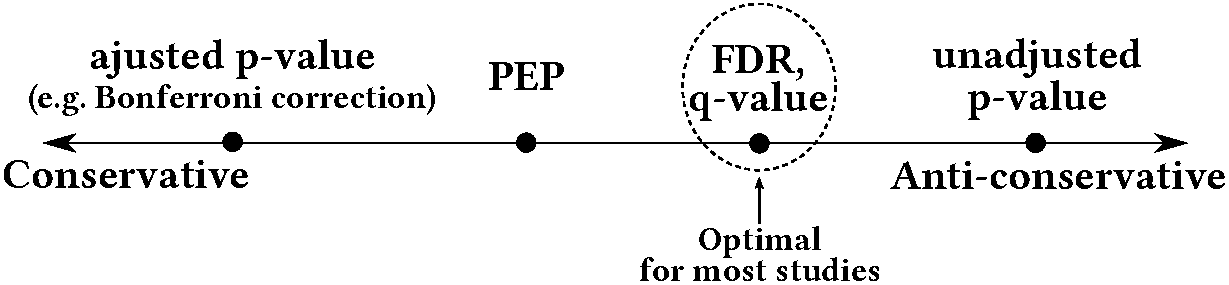
\includegraphics[scale=0.58]{background/MSstatsVal.pdf}\centering
    \vspace{-3mm}
    \caption[Methods for assigning statistical significance]{\label{fig:MSstatval}%
    \textbf{Methods for assigning statistical significance to a collection of \psms}
   --- Adapted from \mycite{Kall2008-tf}.}
\end{figure}

Methods based on \gls{PEP} instead of q-values are more conservative,
as \glspl{PEP} are always greater than q-values~\mycite{Kall2008-tf},
see \Cref{fig:MSstatval}.
For an individual validation,
\eg\ checking the presence of a specific peptide in a particular condition,
\glspl{PEP} are more indicative.
On the other hand, q-values are favoured
where the whole collection of \psms\ is considered,
\eg\ for an overview of the proteome landscape.~\mycite{Kall2008-tf}\mybr\

\subsubsection{Protein inference}\label{subsec:proteinInference}

While identified as the key problem more than fifteen years ago,
protein inference (\ie\ identification) remains
the main challenging issue in shotgun proteomics~\mycite{Nesvizhskii2005-wd,He2016-yi}.
Note that often in the literature,
%as researchers' main interest is
%to identify expressed proteins across samples and conditions,
\emph{protein inference} also encompasses
the peptide identification as an intermediate step
and the results validation
as they influence the protein identification quality.\mybr\

Protein inference consists
in assembling peptides into sets of reliable proteins.
Most assembly algorithms model
the relationship between identified peptides and proteins sequences
as a bipartite graph~\mycite{Huang2012-nr}, illustrated in \Cref{fig:bipartite}.
Proteins identified by two or more (unique) peptides represent the best case:
their identification is reliable and computationally lighter.
However,
the existence of \enquote{degenerate peptides} and
\enquote{one-hit wonder} proteins~\mycite{Huang2012-nr,He2016-yi} makes
this task challenging and computationally intensive.\mybr\

Degenerate peptides are ambiguous peptides
that are shared by multiple protein sequence definitions.
They create a computational challenge
because it is difficult
to solve from which proteins they are derived
and to select which of the two following options is true:
either all the related proteins are expressed in the sample
or only some of them.
Some workflows cluster together proteins with homologous sequences
to ease the process.
More often, to lessen the computational and interpretation burden,
these ambiguous peptides are discarded, and
the inference relies solely on \enquote{unique peptides},
\ie\ peptides that are attributable to one protein sequence only.\mybr\

\enquote{One-hit wonders} are proteins
that are identified by a single peptide only.
They require careful handling regardless of their peptide uniqueness status,
since if the peptide identification is a false positive (\ie\ an artefact),
then the protein is also a false positive.
Shorter proteins,
are generally harder to identify (and quantify)
because many are one-hit wonders.\mybr\

To explain the computational challenges of the peptide assembly,
\citet{Huang2012-nr} propose to start with two assumptions:
(1) all ($m$) peptides are true positive,
and (2) peptides have an equal probability of detectability.
A first assumption corollary is
the presence of many homologous proteins in the sample.\mybr\

Besides, one can derive from the first assumption
that there are a minimal and a maximal value
for the number $n$ of proteins that can be identified
from the set of $m$ peptides.
Returning the exhaustive list of proteins (\ie\ $n_\text{Max}$)
that comprise all $m$ peptides (\eg\ \citet{Tabb2002-wm}) is one possible solution,
but it is much more difficult to calculate the minimal list
(\ie\ $n_\text{min}$) that does the same.
As all the peptides $m$ are supposed to be true,
they have to be included in any of the final minimal list proteins.
Therefore inferring this protein list can be formulated
as a \emph{set covering problem}~\mycite{Cormen2009-rk,Hochbaum1997-db}.
The set covering problem is known to be \gls{NP}-complete~\mycite{Van_Leeuwen1990-sn},
and for which it is in practice impossible to calculate an optimal solution.
Usually, algorithms approximate this solution through a parsimonious approach.\mybr\

Many inference algorithms seek
a compromise between the minimal and exhaustive lists of possible proteins.
While the minimal list probably excludes many true positives
(but can still include false positives),
the exhaustive list is indisputably comprising a large number of false positives
as the parameters are set to maximise the number of peptide/proteins matches;
statistically, a subset of these matches are random.
In the sequence database,
there are many proteins with the same peptidic sequence,
\eg\ a protein $A$, expressed in one set of cells, and
another, $B$, expressed only in another non-overlapping set of cells.
While a sample is only expressing $A$,
an exhaustive solution will also report
$B$ as one of the proteins expressed in the sample.
Statistically,
the greater the size of the reference database
and the expression complexity of the sample,
the greater is the number of false positives in the results
because of the degenerate peptides.\mybr\

On the other hand,
if a peptide is associated to one unique protein in a database
when this peptide is identified with high confidence in a sample,
it is extremely probable that the protein is truly present.
However, these one-hit wonders are also trickier because
the protein presence is reduced to
the probability of the peptide to be a true positive instead of an artefact.
Even a greater number of \gls{MS/MS} spectra supporting a peptide existence
is only the reflection of a remarkably low probability of the protein being absent
in the sample.\mybr\
%\eg of a reason: all proteins may not be properly sequenced or annotated

In this hypothetical setting
where all peptides are true positives and equally likely to be detected,
the inference is already challenging;
it becomes even more complex with real data.
The minimal list can be shorter than the theoretical one as
the identified peptides can be false positives.
On the other hand,
proteomic platforms and pipelines tend to
repeatedly and consistently detect and quantify particular sets of peptides
(\emph{proteotypic} peptides)~\mycite{Mallick2007-za,Bergeron2007-my,Fusaro2009-uc}.
Thus, many peptides are difficult to capture with \ms\ (even with \gls{MS/MS}).
This has two implications.\mybr\

First, many algorithms associate additional information
to the bipartite peptide/protein graph (shown in \Cref{fig:bipartite})
to improve the identification coverage.
The algorithms can exploit different data sources, \eg\ raw and corrected \gls{PSM} scores,
single stage \gls{MS} or raw \gls{MS/MS} spectra,
peptide expression profiles, \mRNA\ expression data,
protein-protein interaction network or gene model.
\citet{Huang2012-nr} propose that additional information can further
extend the exhaustive list of possible proteins.\mybr\

Secondly, the proteotypic peptides have led to
the development of \emph{peptide detectability}~\mycite{Tang2006-qh,Alves2007-ui},
which can help to deal with degenerate peptides
by attributing probabilities to each peptide/protein assignment.
Peptide detectability is considered as a intrinsic peptide property.
It is only determined by the peptide primary sequence and
its location within the protein.\mybr\
%Depending on its chemical groups and their relative sequence,
%the peptide will ionise and fragment more or less;
%peptides situated within protein folds may be more protected,
%so less likely cut out of the protein and then detected.

\begin{figure}[!htb]
    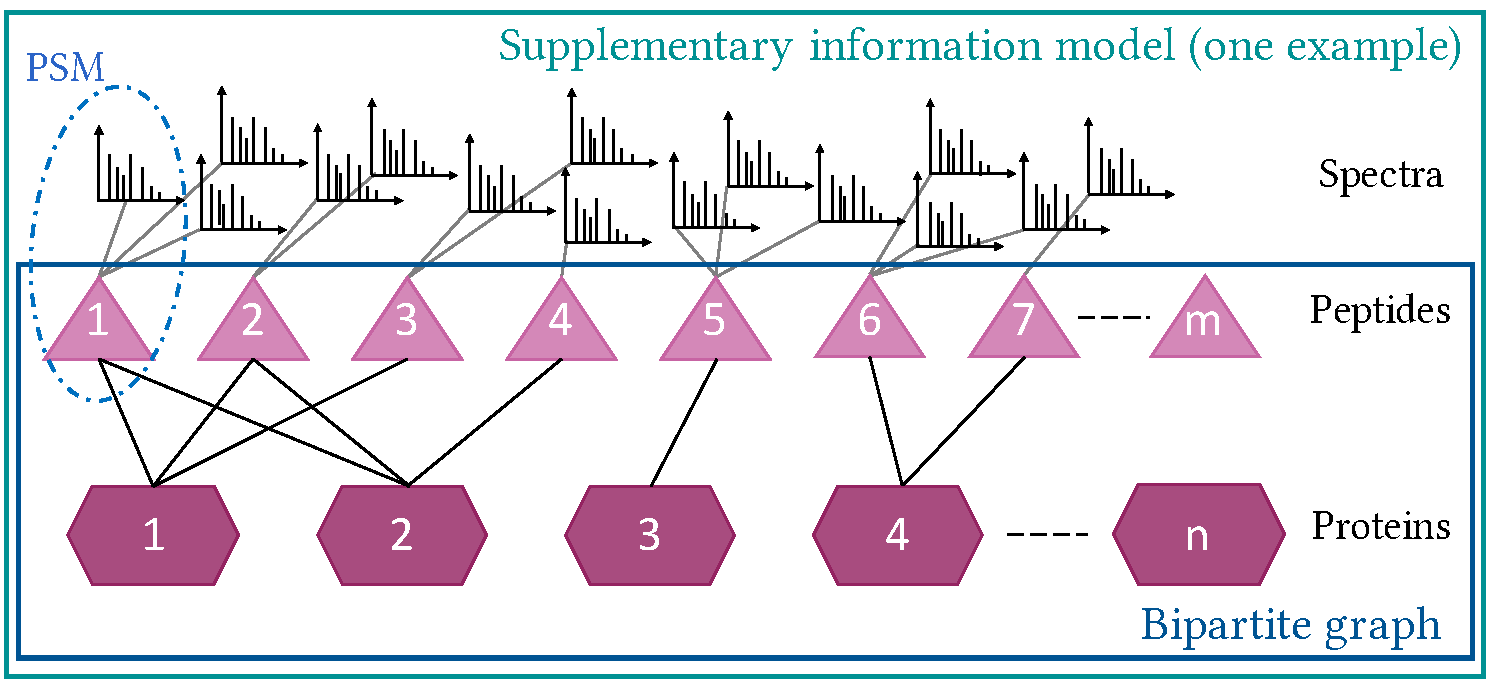
\includegraphics[scale=0.50]{background/modelPeptideAssembly1.pdf}\centering
    \vspace{-0.2mm}
    \caption[Protein inference: the bipartite graph]{\label{fig:bipartite}%
    \textbf{Protein inference: the bipartite graph.} In order to infer proteins,
    algorithms attribute each validated peptide to possible proteins of origins.
    \textit{Peptides 1 and 2} are both included in the definition of
    \textit{proteins 1 and 2};
    it is impossible to determine if both proteins are present in the sample or
    not based on these two peptides only.
    \textit{Peptide 3} backs the existence of \textit{protein 1} and
    \textit{Peptide 4} backs the existence of \textit{protein 2};
    if either \textit{peptide 3} or \textit{peptide 4} is missed in detection,
    it is easy to conclude that only one of \textit{proteins 1 and 2}
    is only present.
    On the other hand, \textit{protein 3} is only identified by \textit{peptide 5}.
    If the latter is an artefact, then \textit{protein 3} is also an artefact.
    In order to achieve the inference,
    peptide assembly algorithms can rely on
    the bipartite graph as sole input (solid blue box),
    or they can include other data types as well,
    \eg\ the score associated to each \gls{PSM} (dashed blue circle) or
    the raw spectra itself (solid teal box).
    }
\end{figure}

\Cref{fig:bipartite} shows how degenerate peptides, one-hit wonder proteins
and the validation quality of the peptide identification
complicate the inference.
Note that if an edge connects a peptide $i$ and a protein $j$,
the peptide $i$ is said to be covered by the protein $j$~\mycite{Huang2012-nr}.
\textit{Protein 1} and \textit{protein 2} share
\textit{peptide 1} and \textit{peptide 2}.
As both \textit{protein 1} and \textit{protein 2} are also covering
another peptide (\textit{peptide 3} for \textit{protein 1}
and \textit{peptide 4} for \textit{protein 2}),
it seems reasonable to assume that both proteins are expressed without more information.
If \textit{peptide 4} is actually a false positive,
would it mean then that only \textit{protein 1} is expressed?
Now, what happens if \textit{peptide 4} is hard to detect and
is missing from the validate list of peptides?
\textit{Peptide 5} is the only one to identify \textit{protein 3}
while \textit{peptide 6} and \textit{peptide 7} are
both backing the existence of \textit{protein 4}.
If one of the two latter peptides is an artefact,
\textit{protein 4} is still most likely a true positive.
However, if \textit{peptide 5} is a false positive,
so is \textit{protein 3}.\mybr\

Many different algorithms tackle this peptide assembly key step.
\citet{Huang2012-nr} organise them in two categorisation frameworks:
one based on the needed search engine for the list of \psms,
the second one (presented in \Cref{fig:ProtInfClass})
based on the underlying algorithmic technique.
Many different approaches and algorithms with their related tools
have been reviewed in the literature~\mycite{Huang2012-nr,Serang2012-jl}.\mybr\

\begin{figure}[!htb]
    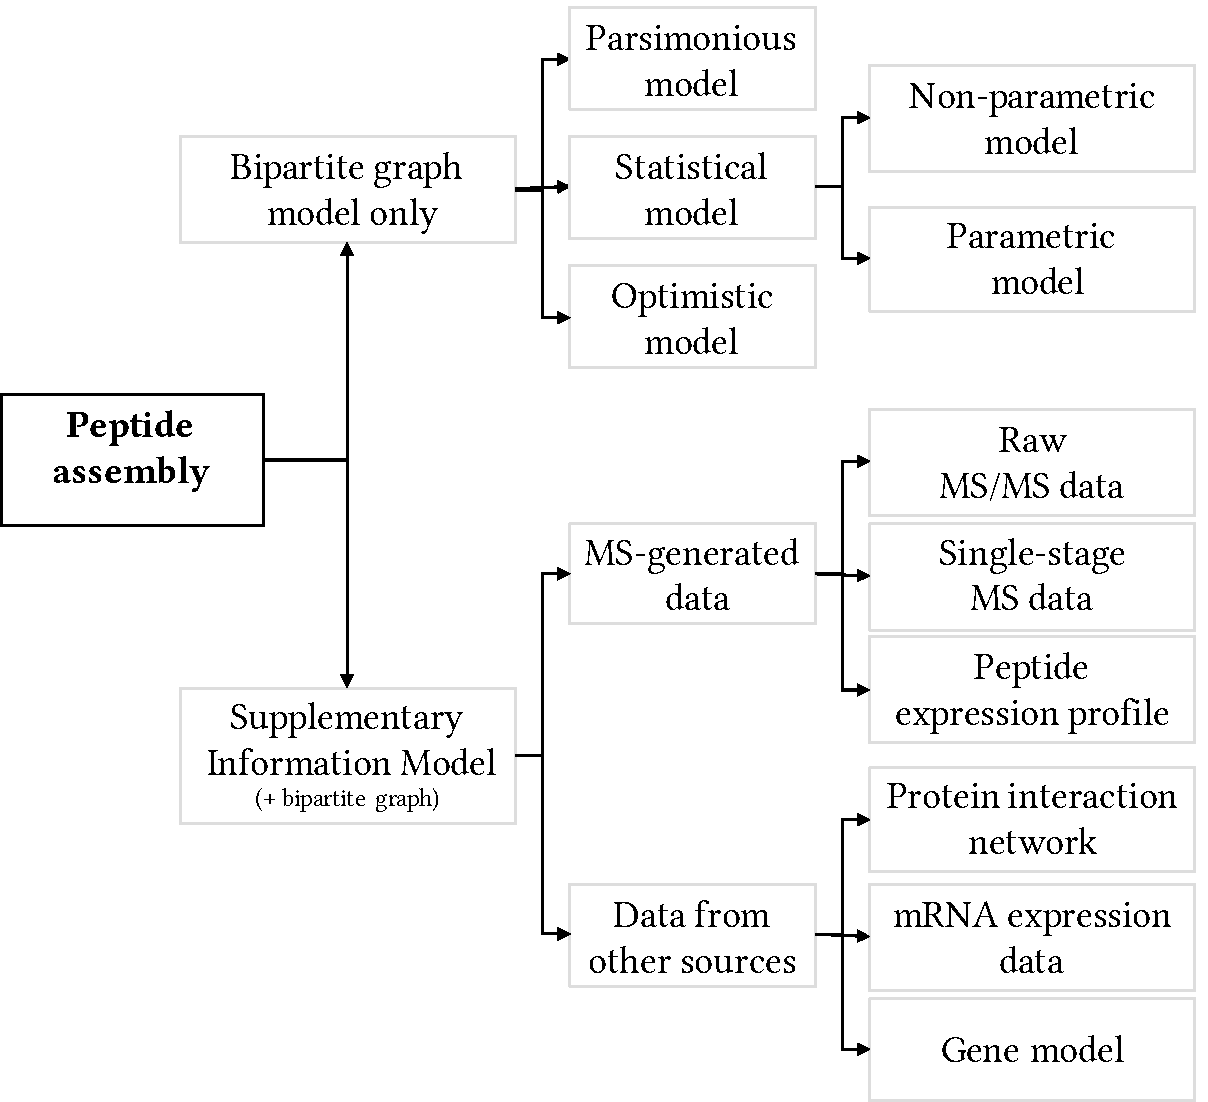
\includegraphics[scale=0.58]{background/ProtInfClass.pdf}\centering
    \caption[Peptide assembly models classification]{\label{fig:ProtInfClass}%
    \textbf{\citet{Huang2012-nr} peptide assembly models classification.}
    }
\end{figure}

Despite the partial or lack of overlap between
sets of confidently identified peptides,
combining several search engines to infer the proteins
has proven to yield better results than a single search~\mycite{Searle2008-dx}.
At worst, it improves the confidence of the identification
as more peptides are characterised per protein~\mycite{Huang2012-nr,Audain2017-jj}.\mybr\

Most analyses benefit from validating the inferred proteins.
Unfortunately,
there is a lack of consensual methodology
to determine a protein \gls{FDR}
and strong opinion divergences on its conceptual validity
in the field~\mycite{Savitski2015-fx}.
A few are even questioning its validity~\mycite{Cottrell2013-ru}.
Beyond the differences due to frequentist and Bayesian definitions and approaches,
part of the pointed out discrepancies~\mycite{The2016-ua} is caused by
overlooking that protein inference tools are concurrently using
two different null hypotheses ($\mathcal{H}_0$ --- see \Cref{H0}).
Two common $\mathcal{H}_0$ statements testing
the validation of a protein identification are:\mybr\
\begin{eqlist}
    \item[$\mathcal{H}_0'$] The best scoring peptide is incorrectly matched
        to the protein.
        (Often, the protein \gls{FDR} is derived from its best scoring peptide.)
    \item[$\mathcal{H}_0''$] The protein is absent from the sample.
\end{eqlist}

Nonetheless, the most widespread method is based on the \gls{TDA}
and the protein \gls{FDR} is computed with \Crefp{eq:fdr-prot}{~}.
\citet{Savitski2015-fx} demonstrate that the \emph{classic} \gls{TDA}
largely overestimate the \gls{FDR} for large datasets.
To overcome this,
\citet{Savitski2015-fx} propose a new \enquote{\emph{picked}} \gls{TDA}.
This approach pairs together target and decoy sequences of each protein
instead of treating them individually.
For each pair, the protein scores of the target and the decoy are compared,
and the highest is kept and the other one discarded.
\citet{The2016-ua} encourage the use of the \enquote{\emph{picked}} \gls{TDA}
when one's analysis is based on $\mathcal{H}_0'$,
but recommend to keep the classical \gls{TDA} for $\mathcal{H}_0''$
as there is a lack of a better method to date
(and \enquote{\emph{picked}} \gls{TDA} actually underestimates it in that case).\mybr\

\subsubsection{Protein quantification (label-free)}\label{subsubsec:protQuantLB}

Label-free quantification methods will most likely improve in the future.
\citet{Nikolov2012-hq} review many of the currently available ones and report that
methods created for label-free absolute quantification experiment designs
can be adapted for relative ones.\mybr\

Spectral/peptide counting is a widespread method.
\citet{Liu2004-cj} present a linear correlation over two magnitude orders
between the relative protein abundance and the acquired spectra number.
Spectral counting is simple and reliable for most proteins
but requires proper normalisation.
Many other methods (\eg\ \softCi{APEX}{apex-tool} or \softCi{emPAI}{emPAI-tool})
are derived thereof.
There are also peak intensity based methods such as \glsentrydesc{IBAQ} (\gls{IBAQ}).
\citet{Arike2012} report that this latter method is better than the previous ones
based on spectral counting as the estimated quantification correlates better to
the absolute abundance.
\citet{TOP3isbetter} refine this statement
as \gls{IBAQ} has biases and quantification errors
that make is unfit for direct
use for a proportional assessment of the complete protein set;
%Where quantifying low abundant proteins is a challenge
%for all the current label-free quantification,
\gls{IBAQ} dramatically underestimates them.
Instead, to improve the general quantification estimation,
%\citet{TOP3isbetter}
they advocate a \emph{Top3} approach~\mycite{Silva-Top3},
which represents the abundance of each protein by the average or sum intensity of
its three best ionised (unique) peptides.
\emph{Top3} allows better quantification of the proteome landscape in general,
even if it is less accurate for the shortest proteins and
saturates for the largest ones.\mybr\

Common normalisations
(\eg\ \gls{NSAF}~\mycite{Zybailov2006-nk}, see \Cref{eq:NSAF}, p.~\pageref{eq:NSAF})
include the length of the protein sequences
(as longer proteins are more likely to produce greater number of peptides and
to be sampled) and the number of spectra that have been acquired within a sample
for each protein.
Similar approaches to \Rnaseq\ can be used to allow protein comparison
across different samples.\mybr\


\section{Possible~downstream~analyses~for~expression~data}\label{sec:enrichmentAnalysis}

\Glspl{ORA} are a standard final stage analysis on expression data.
They can provide biological insights and hint on mechanisms.
\Glspl{ORA} highlight sets of genes (or proteins or metabolites) categories
that are overrepresented in a selected subset of the data
compared to the expectation of a random category.
Many expression studies aim to produce \textquote{a list of \enquote{interesting}
biomolecules}~\mycite{Tipney2010-mz},
\glspl{ORA} help to determine the most pertinent ones
by providing biological context and increasing statistical power.
Besides, such lists are often substantial
so extracting common functional information from subsets of genes/proteins eases
the interpretation of the data.
Various tools and algorithms have been developed
to overcome the daunting task of individually checking the genes/proteins.
See \citet{Shi_Jing2015-yh} for some examples.
While, the field has been reviewed a few times
(see \citet{Khatri2005-su,Huang2009-zk,Khatri2012-ki}),
it is still unfortunately lacking a gold standard
and systematic comparative studies~\mycite{Mathur2018-ph}.\mybr\

Depending on the experimental design and study,
the list of biomolecules can be associated with a rank or another form of a score.
As \glspl{DEA} are the most widespread type of analyses for expression data,
many tools and algorithms work solely with the corresponding outputs.
Hence, those are unfit for other types of studies
(such as the ones in this thesis).
Available \gls{gsea}~\mycite{Subramanian2005-kd} tools are commonly inadequate
for any other purpose than \gls{DEA} studies.
See \citet{Tamayo2012-qw,Irizarry2009-sc}
and the included references for some examples of \gls{gsea} tools.\mybr\

On the other hand, while still devised for \gls{DEA},
other tools handle any rank or score and thus are more flexible;
they can analyse data outside of their original scope.
Many \gls{go} analysis tools fall into this latter category.\mybr\

\subsection{GO analysis (GOA)}\label{sec:goaGeneralities}
The \gls{go} is a collaborative and curated classification
that describes the gene products
following three hierarchically structured and controlled vocabularies
(also known as ontologies):
either based on the biological processes (\enquote{BP}) to which they contribute,
their position (when active) in the cell (cellular component (\enquote{CC})) or
their biochemical activity, \ie\ molecular function (\enquote{MF}).~\mycite{Ashburner2000-by}\mybr\

Generally, \glspl{goa} compare a selected list (with the genes/proteins of interest)
to a background list
(\eg\ all observed genes in the experiment or all existing genes in the annotation).
For each \gls{go} term,
this method computes the enrichment of the selected set based on
the real fraction of the set for the considered \gls{go} term and its likelihood
(computed on the background list).
For example, if for a \gls{go} term $\mathcal{A}$ is associated with 0.1\%
of all the background (list) genes,
but then over 70\% of the genes from the selected list are associated
with \gls{go} term $\mathcal{A}$,
one can safely accept that the selected genes list is enriched for this term.
The various tools rely on different statistical tests to determine
if the enrichments are significant.
Investigating only a few \gls{go} terms of interest is common.\mybr\

While ranked lists are unnecessary for \glspl{goa},
one can apply a cut-off before running this type of analysis.
However, in those cases,
\gls{gsea} will be generally favoured to a \gls{goa}.\mybr\

\section{Reproducibility~and~Experimental~design}\label{sec:expDesign}

Science develops on reproducible facts,
as they help with drawing relevant and accurate conclusions.
To increase reproducibility,
it is essential that observations and measurements
be (as much as possible) unbiased
towards any parameter outside of the study focus.
To this aim, one of the critical issues that need to be tightly monitored
is the presence of \emph{batch effects}.
Including \emph{replicates} in the study is the most effective way to control
for the unwanted batch effects.\mybr\

Another issue is due to high-throughput transcriptomics and proteomics
still being evolving fields.
For each new identified problem,
researchers create new tools and algorithms.
However, these are often aimed to one study only
and their reuse in another study can be difficult,
or even impossible (\eg\ discontinued proprietary software).
On the other hand, well established tools allow fine tuning many parameters,
which impact can be overlooked while the reporting.
Thus, it is unsurprising that result agreements between different tools
are unsatisfactory~\mycite{reviewRNAseqBestpractice}.\mybr\

\subsection{Batch effects}\label{sub:BatchEffect}

Batch effects are artefactual and due to all the variables
that the investigator can not control
(either by lack of technology, design or knowledge), for example,
environmental conditions, reagent or sample lots,
genetic population background or experimenters.
They are often the source of complication for many studies
(including high-throughput genomic ones)~\mycite{batchEffect}.\mybr\

The danger lies in overlooking them and then confounding these artefacts
with biological results, which will lead to flawed interpretation and conclusions.
Several studies have been refuted in the past because of unaccounted batch effects.
Usually, issues in the initial results are detected by others laboratories,
which notice high correlations between the \enquote{biological} findings
of the original study and the running dates or processing groups.
Thus, questions on the biological validity arise.\mybr\

The first step to address them is through well-designed experiments~\mycite{batchEffect},
which include technical and biological replicates.
These replicates are usually created and randomly processed
as to avoid creating any artefactual link between them.
A replicate is a set of measurements done in the same condition.\mybr\

Correction can be applied and may help resolve batch effects in some cases.
For examples, see \citet{Oytam2016-rb,Gagnon-Bartsch2012-dj,Peixoto2015-wg}.\mybr\

\subsection{Technical replicates}
Technical replicates are initially from the same sample,
which has been tested multiple times through a given experimental protocol.
It allows testing for the variability of the protocol itself.
While using the same sample to test different protocols
may also be referred to as \enquote{technical},
it is better to avoid this appellation as this creates confusion.\mybr\

\subsection{Biological replicates}
Biological replicates are testing the same cells or tissues from different individuals
through the same protocol.
They allow assessing the biological variability
(which is higher than the technical variability, since it also encompasses it).\mybr\

\subsection{Study design example: meta-analyses}

Meta-analyses are studies that combine (or aggregate) the results of multiple analyses.
One of their main weaknesses is
that meta-analyses lack
to control bias sources and correct for bad designs~\mycite{Slavin1986-py}.
Because results from smaller studies are more prone to \enquote{play of chance},
they are usually weighted less than bigger studies
when they are directly combined across many studies~\mycite{Egger1997-ny},
particularly when combining statistical results.
However, it is not always true and bigger studies may be subjected
to greater uncontrolled variations.
\citet{Egger1997-ny} recommend testing the heterogeneity across the studies
to be combined.
Examining the studies outcomes' similarity degree allows figuring out
if the variation between the studies is only due to sampling or
to a distribution of different effects.
In order to compare studies together,
individual results are standardly expressed
(\eg\ means, confidence interval).\mybr\


\section{Discussion and conclusion}\label{sec:bgConcl}

Over the years, the central dogma of molecular biology
has been being refined and better understood.
However, as the first apparent linearity of the theory tends to persist,
so are many assumptions.
For example,
all (or almost all) information necessary to explain the \gls{phenotype} is in the cell;
in its genome and edits provided by
its transcription and translation regulatory mechanisms
that may be triggered by environmental stimuli.
Another assumption is that
\mRNA\ and protein levels should share overall strong correlation coefficients.
Alternatively, as our genomes are so similar,
our transcriptomes and proteomes should also share many similarities.
Although the truth seems more intricate,
these assumptions remain
as we still lack the technical means to test them to their fullest.\mybr\

Due to the intrinsic nature of \gls{DNA}, \mRNAs\ and proteins,
high-throughput \gls{DNA} and \gls{RNA} studies are more well-established
and standardised than proteomic studies.
Although, the study of the genome is the most mature,
it fails to contextualise the phenotype,
especially for non-disease cases
(often referred to as healthy or normal conditions in this thesis).\mybr\

Proteins are in theory the best candidates to study the phenotype.
Unfortunately, high-throughput protein studies
such as shotgun \ms\ are particularly challenging.
The proteins physicochemical diversity and
the lack of technology to amplify proteomes mean that
in order to optimise their studies many different protocols and experimental designs
had to be developed to reach the different proteins in a sample.\mybr\

Since the transcriptome has a dynamic dimension like the proteome
and is technically easier to explore and quantify,
its study has emerged as a reasonable trade-off strategy.\mybr\

